% autosam.tex
% Annotated sample file for the preparation of LaTeX files
% for the final versions of papers submitted to or accepted for 
% publication in AUTOMATICA.

% See also the Information for Authors.

% Make sure that the zip file that you send contains all the 
% files, including the files for the figures and the bib file.

% Output produced with the elsart style file does not imitate the
% AUTOMATICA style. The style file is generic for all Elsevier
% journals and the output is laid out for easy copy editing. The
% final document is produced from the source file in the
% AUTOMATICA style at Elsevier.

% You may use the style file autart.cls to obtain a two-column 
% document (see below) that more or less imitates the printed 
% Automatica style. This may helpful to improve the formatting 
% of the equations, tables and figures, and also serves to check 
% whether the paper satisfies the length requirements.

% Please note: Authors must not create their own macros.

% For further information regarding the preparation of LaTeX files 
% for Elsevier, please refer to the "Full Instructions to Authors" 
% from Elsevier's anonymous ftp server on ftp.elsevier.nl in the
% directory pub/styles, or from the internet (CTAN sites) on
% ftp.shsu.edu, ftp.dante.de and ftp.tex.ac.uk in the directory
% tex-archive/macros/latex/contrib/supported/elsevier.


%\documentclass{elsart}               % The use of LaTeX2e is preferred.

\documentclass[twocolumn]{autart}    % Enable this line and disable the 
                                     % preceding line to obtain a two-column 
                                     % document whose style resembles the
                                     % printed Automatica style.
\usepackage{natbib}
\usepackage{amssymb}
\usepackage{amsmath}
\usepackage{graphicx}
\usepackage{comment}
\usepackage{booktabs}
%\usepackage{breqn}
\usepackage{bm}
\usepackage{graphicx}
\usepackage{epstopdf}
\setcounter{MaxMatrixCols}{20}
\usepackage{amssymb}
\usepackage{wasysym}
\usepackage{float}
\usepackage{color}
\usepackage{dsfont}
\usepackage{algorithm,algorithmicx}
\usepackage{algpseudocode}
\usepackage{epstopdf}
\usepackage{tabularx}
%\usepackage{cite}
\usepackage{enumitem}
\usepackage{marginnote}
\usepackage{graphicx}          % Include this line if your 
                               % document contains figures,
%\usepackage[dvips]{epsfig}    % or this line, depending on which
                               % you prefer.
\newcommand{\eod}{\ensuremath{\hfill\Box}}
\begin{document}

\begin{frontmatter}
%\runtitle{Insert a suggested running title}  % Running title for regular 
                                              % papers but only if the title  
                                              % is over 5 words. Running title 
                                              % is not shown in output.

\title{Event-triggered Partitioning for Non-centralized Predictive-Control-based Economic Dispatch of Interconnected Microgrids: Technical Report\thanksref{footnoteinfo} \vspace{-20pt}} % Title, preferably not more 
                                                % than 10 words.

\thanks[footnoteinfo]{%This paper was not presented at any IFAC 
%meeting. 
Corresponding author W.~Ananduta.}

\author[delft]{Wicak Ananduta}\ead{w.ananduta@tudelft.nl},    % Add the 
%\author[asu]{Angelia Nedi\'{c}}\ead{angelia.nedich@asu.edu},               % e-mail address 
\author[iri]{Carlos Ocampo-Martinez}\ead{carlos.ocampo@upc.edu}  % (ead) as shown
\address[delft]{Delft Center for Systems and Control, TU Delft}
\address[iri]{Automatic Control Department, Universitat Polit\`{e}cnica de Catalunya}  % Please supply                                              
%\address[asu]{School of Electrical, Computer and Energy Engineering, Arizona State University}             % full addresses

          
\begin{keyword}                           % Five to ten keywords,  
	complex system management, large-scale complex systems, system partitioning, control of networks, decentralisation, real time simulation and dispatching, non-centralized MPC 						              % chosen from the IFAC 
\end{keyword}                             % keyword list or with the 
                                          % help of the Automatica 
                                          % keyword wizard


\begin{abstract}                          % Abstract of not more than 200 words.
A non-centralized model predictive control (MPC) scheme for solving an economic dispatch problem of electrical networks is proposed in this paper. The scheme consists of two parts. The first part is an event-triggered repartitioning method that splits the network into a fixed number of non-overlapping sub-systems {(microgrids)}. The objective of the repartitioning procedure is to obtain self-sufficient microgrids, i.e., those that can meet their local loads using their own generation units. However, since the algorithm does not guarantee that all the resulting microgrids are self-sufficient, the microgrids that are not self-sufficient must then form a coalition with some of their neighboring microgrids. This process becomes the second part of the scheme. By performing the coalition formation, we can decompose the economic dispatch problem of the network into coalition-based sub-problems such that each subproblem is feasible. Furthermore, we also show that the solution obtained by solving the coalition-based sub-problems is a feasible but sub-optimal solution to the centralized problem. Additionally, some numerical simulations are also carried out to show the effectiveness of the proposed method.  
\end{abstract}

\end{frontmatter}

\section{Introduction}
%!TEX root = paper.tex


This paper follows in a long line of investigation of the following Ramsey-type graph colouring problem.
\begin{quote}\em
What is the best upper bound on the chromatic number $\chi$ for graphs of given maximum degree $\Delta$ and given maximum local density --- that is, with neighbourhood subgraphs each inducing at most a certain edge density?
\end{quote}
This deep and elegant problem has its roots going back more than half a century~\cite{Viz68}.
The archetypal result of this type is one of Johansson~\cite{Joh96} that was recently sharpened with the entropy compression method by Molloy~\cite{Mol19} as follows: any graph $G$ that is triangle-free --- that is, with a maximum local density of precisely zero --- has chromatic number satisfying $\chi(G)\le(1+o(1))\Delta(G)/\log\Delta(G)$ as $\Delta(G)\to\infty$.
This betters by a logarithmic factor the trivial upper bound $\chi(G)\le \Delta(G)+1$ that holds for {\em any} graph $G$.
It is sharp up to a (small) constant multiple due to random regular graphs.
Alon, Krivelevich and Sudakov~\cite{AKS99} showed a more general bound under the condition of maximum local density at most $1/f=o(1)$. This too has been refined recently~\cite{DKPS20+} (cf.~also~\cite{DJKP18+} and~\cite{DKPS20+b}) as follows: any graph $G$ with local density at most $1/f$, where $f=f(\Delta(G))$, $f \to\infty$ as $\Delta(G)\to\infty$, and $f\le \binom{\Delta(G)}2+1$, has chromatic number satisfying $\chi(G)\le(1+o(1))\Delta(G)/\log\sqrt{f}$. Note that this statement includes the triangle-free one as a special case with $f=\binom{\Delta(G)}2+1$. While in that result the condition $1/f=o(1)$ excludes the possibility of a neighbourhood subgraph having non-negligible density, here it is this `denser' situation which will be our primary focus.


To specify how far we are from a trivial local density condition, we adopt the following notation. Given $\sigma>0$, a graph $G$ is said to be {\em $\sigma$-sparse} if for every $v\in V(G)$ the subgraph $G[N(v)]$ induced by the neighbourhood $N(v)$ of $v$ has at most $(1-\sigma)\binom{\Delta(G)}2$ edges.
As a means towards progress in a problem of Erd\H{o}s and Ne\v{s}et\v{r}il (of which we discuss in further detail later on in the paper), Molloy and Reed~\cite{MoRe97} initiated the study of the chromatic number of $\sigma$-sparse graphs. In particular, using a ``na\"ive'' probabilistic colouring procedure, they showed the following.

\begin{theorem}[Molloy and Reed~\cite{MoRe97}]\label{thm:MoResparse}
There is a positive function $\eps_{\ref{thm:MoResparse}}=\eps_{\ref{thm:MoResparse}}(\sigma)$ such that the following holds.
For each $0<\sigma\le1$ there is $\Delta_0$ such that the chromatic number satisfies $\chi(G)\le (1-\eps_{\ref{thm:MoResparse}})\Delta(G)$ for any $\sigma$-sparse graph $G$ with $\Delta(G)\ge\Delta_0$.
\end{theorem}
\noindent
Note this constitutes a constant factor improvement upon the trivial upper bound in this case.

Our work marks important progress in the quantitative optimisation of Theorem~\ref{thm:MoResparse} for $\sigma$-sparse graphs, i.e.~in pursuit of the maximum $\eps_{\ref{thm:MoResparse}}$ as a function of $\sigma$. We briskly survey the landscape prior to our work. Molloy and Reed themselves proved Theorem~\ref{thm:MoResparse} for 
$\eps_{\ref{thm:MoResparse}} \ge 0.0238\sigma$.
It was over two decades before Bruhn and Joos~\cite{BrJo18} were able to improve upon this by establishing that 
$\eps_{\ref{thm:MoResparse}} \ge 0.1827\sigma-0.0778\sigma^{3/2}$.
Soon after, Bonamy, Perrett and Postle~\cite{BPP18+} improved this further through an iterative approach (that also captured the more general notions of list and correspondence colouring), and showed that  
$\eps_{\ref{thm:MoResparse}} \ge 0.3012\sigma-0.1283\sigma^{3/2}$.
Our contribution is the analysis of an improved colouring procedure based on random priority assignment that shows Theorem~\ref{thm:MoResparse} is true for any 
$\eps_{\ref{thm:MoResparse}} < \sigma/2 - \sigma^{3/2}/6$.
\begin{theorem}
\label{col_result}
Define $\eps_{\ref{col_result}} = \eps_{\ref{col_result}}(\sigma) = \sigma/2 - \sigma^{3/2}/6$.
For each $\iota>0$ and $0<\sigma\le1$, there is $\Delta_{\ref{col_result}}=\Delta_{\ref{col_result}}(\iota)$ such that the chromatic number satisfies $\chi(G)\le (1-\eps_{\ref{col_result}}(\sigma)+\iota)\Delta(G)$ for any $\sigma$-sparse graph $G$ with $\Delta(G)\ge\Delta_{\ref{col_result}}$.
\end{theorem}

\noindent
In the densest cases, as $\sigma\to0$, the leading coefficient $1/2$ in the expression for $\eps_{\ref{col_result}}$ is best possible, as certified by the following simple construction, cf.~also~\cite[Ex.~10.1]{MoRe02}.

\begin{proposition}\label{prop:sharp}
For each $\Delta\ge 1$ and  $\sigma>0$, there is a $\sigma$-sparse graph $G^\Delta_\sigma$ of maximum degree $\Delta$ such that as $\sigma\to0$ its chromatic number satisfies
\(
1-\chi(G^\Delta_\sigma)/\Delta = \sigma/2+o(\sigma^{3/2}).
\)
\end{proposition}
\begin{proof}
Let $G^\Delta_\sigma$ consist of a clique of size $\min\{1,\lfloor\sqrt{1-\sigma}\cdot\Delta\rfloor\}$ with $\Delta+1-\min\{1,\lfloor\sqrt{1-\sigma}\cdot\Delta\rfloor\}$ vertices of degree one appended to each vertex in the clique. It is trivial to verify that this graph has maximum degree $\Delta$, is $\sigma$-sparse, and has chromatic number $\min\{1,\lfloor\sqrt{1-\sigma}\cdot\Delta\rfloor\}$. The conclusion follows from a Taylor expansion of $1-\sqrt{1-\sigma}$ at $\sigma=0$.
\end{proof}

\noindent
On the other hand, in the sparser cases one might hope for a guarantee on $\eps_{\ref{thm:MoResparse}}(\sigma)$ that approaches $1$ as $\sigma\to1$, since Johansson's result for triangle-free graphs implies in the special case $\sigma=1$ that Theorem~\ref{thm:MoResparse} holds for any $\eps_{\ref{thm:MoResparse}}(1) < 1$. Thus there is still room for improvement, since the methods we have employed here only imply for that special case that Theorem~\ref{thm:MoResparse} holds for any $\eps_{\ref{thm:MoResparse}}(1) < 1/3$.

Nevertheless Theorem~\ref{col_result} yields state-of-the-art bounds in two well-known and longstanding graph colouring conjectures, namely the Erd\H{o}s--Ne\v{s}et\v{r}il conjecture and Reed's conjecture.
In Subsections~\ref{sub:ErdosNesetril} and~\ref{sub:Reed}, we discuss these consequences.

The proof of Theorem~\ref{col_result} is quite technical and involved, and is provided in full in Section~\ref{sec:proof}.
For the convenience of the reader, we have prefaced Section~\ref{sec:proof} with a succinct overview of the ideas and methods.

\subsubsection*{Structure of the paper}

Subsections~\ref{sub:ErdosNesetril} and~\ref{sub:Reed} describe the background to the Erd\H{o}s--Ne\v{s}et\v{r}il and Reed's conjectures, respectively, and the progress we obtain through Theorem~\ref{col_result}.
Subsection~\ref{sub:prelim} lists some notation and tools we use.
We give an outline of the proof of Theorem~\ref{col_result} at the beginning of Section~\ref{sec:proof}.
The remainder of Section~\ref{sec:proof} provides the full proof.
In Section~\ref{sec:applications}, we give details of the two applications of Theorem~\ref{col_result}.


\subsection{A step towards the Erd\H{o}s--Ne\v{s}et\v{r}il conjecture}\label{sub:ErdosNesetril}


Given a graph $G$, an {\em induced matching} is a subset $M$ of the edges of $G$ such that for any pair $e,e'$ of distinct edges of $M$, neither $e$ and $e'$ are incident nor are any of the four possible edges between an endpoint of $e$ and an endpoint of $e'$ present in $G$.
A {\em strong edge-colouring} of $G$ is a partition of its edge set $E(G)$ into induced matchings of $G$.
The strong chromatic index $\xs(G)$ of $G$ is the least number of parts needed in any strong edge-colouring of $G$. Equivalently, $\xs(G)$ is the chromatic number $\chi(L(G)^2)$ of the square $L(G)^2$ of the line graph $L(G)$ of $G$. (The square of a graph is obtained from the graph itself by adding edges between all pairs of distinct non-adjacent vertices that are connected by a two-edge path.)
In the 1980s (cf.~\cite{Erd88}), Erd\H{o}s and Ne\v{s}et\v{r}il proposed the problem of bounding $\xs(G)$ in terms of the maximum degree $\Delta(G)$ of $G$. Since the maximum degree $\Delta(L(G)^2)$ of the square of the line graph of $G$ is at most $2\Delta(G)(\Delta(G)-1)$, the strong chromatic index is trivially bounded by $\xs(G)\le 2\Delta(G)^2-2\Delta(G)+1$. They conjectured something much stronger.

\begin{conj}[Erd\H{o}s and Ne\v{s}et\v{r}il, cf.~\cite{Erd88}]\label{conj:ErNe}
The strong chromatic index satisfies $\xs(G)\le 1.25\Delta(G)$ for all $G$.
\end{conj}

\noindent
(See~\cite{JKP19} for a fascinating strengthened, yet equivalent, form of this conjecture.)
If true, this bound would be exact for a suitable blow-up of the 5-edge cycle (in the $\Delta(G)$ even case).
It was more than a decade before a breakthrough by Molloy and Reed~\cite{MoRe97}, yielding some absolute constant $\eps>0$ such that $\xs(G)\le (2-\eps)\Delta(G)$ for all $G$.
More specifically, they proved the following statement.

\begin{theorem}[Molloy and Reed~\cite{MoRe97}]\label{thm:MoRestrong}
There is some $\eps_{\ref{thm:MoRestrong}}>0$ and some $\Delta_0$ such that the strong chromatic index satisfies $\xs(G)\leq (2-\eps_{\ref{thm:MoRestrong}})\Delta(G)^2$ for any graph $G$ with $\Delta(G)\ge \Delta_0$.
\end{theorem}

\noindent
(We may bound the absolute constant $\eps>0$ mentioned before by comparing the bound of Theorem~\ref{thm:MoRestrong} with the trivial bound on $\xs(G)$ for those $G$ with $\Delta(G)<\Delta_0$.)
Molloy and Reed proved that $\eps_{\ref{thm:MoRestrong}} \ge 0.001$.
A key insight they made in their proof of Theorem~\ref{thm:MoRestrong} was to split the task into two separate subtasks, first, showing for some absolute constant $\sigma>0$ that $L(G)^2$ is $\sigma$-sparse for all $G$, and, second, showing a nontrivial improvement on the trivial colouring bound under the assumption of $\sigma$-sparsity, i.e.~Theorem~\ref{thm:MoResparse}.
Bruhn and Joos~\cite{BrJo18} were the first to revisit this problem, and they not only significantly improved on the estimate of $\eps_{\ref{thm:MoResparse}}$ in Theorem~\ref{thm:MoResparse} as mentioned earlier, but also proved an asymptotically extremal lower bound on $\sigma>0$ such that $L(G)^2$ is $\sigma$-sparse for all $G$. In this way, they obtained that $\eps_{\ref{thm:MoRestrong}} \ge 0.070$.
The more recent work of Bonamy {\em et al.}~\cite{BPP18+} obtained further improvements. As mentioned earlier, they improved the estimate of $\eps_{\ref{thm:MoResparse}}$ in Theorem~\ref{thm:MoResparse} through an iterative approach. They were moreover able to improve on the separation into two subtasks, by showing better sparsity on a subgraph of $L(G)^2$ according to a degeneracy-type argument. Through this, they obtained that $\eps_{\ref{thm:MoRestrong}} \ge 0.165$.
By combining Theorem~\ref{col_result} with this last-mentioned method, we derive that $\eps_{\ref{thm:MoRestrong}} \ge 0.228$. The proof is given in Subsection~\ref{sub:ErdosNesetrilproof}.

\begin{theorem}
\label{strong_bound}
There is some $\Delta_0$ such that the strong chromatic index satisfies $\xs(G)\leq 1.772\Delta(G)^2$ for any graph $G$ with $\Delta(G)\ge \Delta_0$.
\end{theorem}

\noindent
We humbly agree that the above sequence of improvements on estimates for $\eps_{\ref{thm:MoRestrong}}$ suggests that the hypothetically optimal determination $\eps_{\ref{thm:MoRestrong}}=0.75$ remains far from reach. Even a proof of $\eps_{\ref{thm:MoRestrong}}=0.75$ would leave open the nontrivial task of proving Conjecture~\ref{conj:ErNe} for all graphs with maximum degree less than $\Delta_0$. Despite considerable efforts, so far it has only been established for graphs of maximum degree $3$~\cite{And92,HQT93}.




\subsection{A step towards Reed's conjecture}\label{sub:Reed}

Another Ramsey-type problem (perhaps even closer to quantitative Ramsey theory) asks the following.
\begin{quote}\em
What is the best upper bound on the chromatic number $\chi$ for graphs of given maximum  degree $\Delta$ and given clique number $\omega$?
\end{quote}

\noindent
An aforementioned result of Johansson~\cite{Joh96} has settled this question up to a constant multiple as $\Delta\to\infty$ when $\omega=2$. Already the case $\omega=3$ is open and difficult. This is closely related to an important conjecture of Ajtai, Erd\H{o}s, Koml\'os and Szemer\'edi~\cite{AEKS81}. For $\omega$ asymptotically smaller than $\Delta$ (as $\Delta\to\infty$), the current best bounds were recently obtained in~\cite{DKPS20+}. Again, here we will be mostly concerned with a `denser' regime, namely, when $\omega$ is linear in $\Delta$. Related to this, Reed proposed an evocative conjecture.

\begin{conj}[Reed~\cite{Ree98}]\label{conj:Ree98}
The chromatic number satisfies $\chi(G) \le \lceil \frac12(\omega(G)+\Delta(G)+1)\rceil$ for any graph $G$.
\end{conj}

\noindent
In other words, he asked if the chromatic number $\chi(G)$ of a graph $G$ is always at most the average, rounded up, of the trivial lower bound, $\omega(G)$, and the trivial upper bound, $\Delta(G)+1$, for $\chi(G)$.
If true, the bound is sharp, for instance, for the Chv\'atal graph. The bound is trivially true when $\omega(G)\ge\Delta(G)$ and it follows from Brooks' theorem~\cite{Bro41} for $\omega(G)=\Delta(G)-1$. 
In~\cite{DKPS20+}, it was shown that, if $\omega(G) \le \Delta(G)^c$ for some fixed $c<1/100$, then the bound holds provided $\Delta(G)$ is sufficiently large. (There is some room in the method there to increase the constant $1/100$ slightly, but not above $1/16$ without additional ideas.)
Curiously, despite Johansson's result, the conjecture is still open in the special case $\omega(G)=2$, particularly for small values of $\Delta(G)$.
As evidence towards his conjecture, Reed succeeded in proving, through a lengthy set of arguments that are probabilistic in nature, the following.

\begin{theorem}[Reed~\cite{Ree98}]\label{thm:Ree98}
There is some $\eps_{\ref{thm:Ree98}}>10^{-8}$ and some $\Delta_{\ref{thm:Ree98}}$ such that the chromatic number satisfies $\chi(G) \le \frac12(\omega(G)+\Delta(G)+1)$ for any graph $G$ satisfying $\omega(G) \ge (1-\eps_{\ref{thm:Ree98}})\Delta(G)$ and $\Delta(G)\ge \Delta_{\ref{thm:Ree98}}$.
\end{theorem}

\noindent
Note that this statement implies that some (barely) nontrivial convex combination of $\omega(G)$ and $\Delta(G)+1$ suffices as an upper bound for $\chi(G)$.

\begin{cor}\label{cor:Ree98}
There is some $\eps_{\ref{cor:Ree98}}\ge \eps_{\ref{thm:Ree98}}/2$ and some $\Delta_0$ such that the chromatic number satisfies  $\chi(G) \le \lceil (1-\eps_{\ref{cor:Ree98}})(\Delta(G)+1)+\eps_{\ref{cor:Ree98}}\omega(G)\rceil$ for any graph $G$ with $\Delta(G)\ge \Delta_0$.
\end{cor}

\noindent
Reed himself made little effort to optimise the value of $\eps_{\ref{cor:Ree98}}$, but noted that it cannot be more than $1/2$ by a standard probabilistic construction.
Bonamy {\em et al.}~\cite{BPP18+} recently revisited this problem and showed $\eps_{\ref{cor:Ree98}} > 0.038$. Delcourt and Postle~\cite{DePo17} have announced that $\eps_{\ref{cor:Ree98}} > 0.076$. One consequence of Theorem~\ref{col_result} is an improvement on these estimates, in particular, that $\eps_{\ref{cor:Ree98}} \ge 0.199$. The proof is given in Subsection~\ref{sub:Reedproof}.

\begin{theorem}
\label{Reed_bound}
There is some $\Delta_0$ such that the chromatic number satisfies $\chi(G) \le \lceil 0.801(\Delta(G)+1)+0.199\omega(G)\rceil$ for any graph $G$ with $\Delta(G)\ge \Delta_0$.
\end{theorem}











\section{Problem formulation}
\label{sec:prob_form}
%In this section, we present the MPC-based economic dispatch problem that we consider and provide the outline of the proposed methodology.

%\subsection{Economic dispatch problem}
%\paragraph*{Graph representation of the network}
%We formulation of the economic dispatch problem is provided, following the model of the network. 

Let a distribution power network be represented by the undirected and connected graph $\mathcal{G}=(\mathcal{N},\mathcal{E})$, where the set of busses is denoted by $\mathcal{N}=\{1,2,\dots,n\}$ and the set of edges that connect the busses is denoted by $\mathcal{E}$, i.e., $\mathcal{E}=\{(i,j):i,j\in\mathcal{N} \}\subseteq\mathcal{N}\times\mathcal{N}$. Furthermore, the set of neighbor busses of bus $i$ is denoted by $\mathcal{N}_i$, i.e., $\mathcal{N}_i = \{j:(i,j)\in \mathcal{E} \}$. Each bus $i$ might contain an aggregate load (power demand), dispatchable or nondispatchable distributed generation units, and energy storage devices. Each of these components has operational constraints, which are assumed to be polyhedral and compact. Furthermore, each bus $i \in \mathcal{N}$ also considers power balance equations that must be satisfied  at each iteration $k$, as follows: 
\begin{align}
u^{\mathrm{g}}_{i,k} + u^{\mathrm{st}}_{i,k} + u^{\mathrm{m}}_{i,k} + \sum_{j \in \mathcal{N}_i} v^{j}_{i,k} - {d}_{i,k}=0,  \label{eq:lo_pb}\\
v^{j}_{i,k} + v^{i}_{j,k} = 0, \quad \forall j \in \mathcal{N}_i, \label{eq:coup_pb}
\end{align}
where  ${u}_{i,k}^{\mathrm{g}}\in \mathbb{R}$, $u^{\mathrm{st}}_{i,k}\in \mathbb{R}$, and $u_{i,k}^{\mathrm{m}} \in \mathbb{R}_{\geq 0}$ denote the power generated from dispatchable unit, delivered from/to storage unit, and imported from the main grid if connected, respectively.  %Note that bus $i$ belongs to the set of busses that are connected to the main grid, denoted by $\mathcal{N}^{\mathrm{m}}$, and 
Furthermore, $d_{i,k}\in \mathbb{R}$ denotes the difference between uncertain loads and the power generated from non-dispatchable units, which is also uncertain. Additionally, $v_{i,k}^{j} \in \mathbb{R}$ denotes the power transferred to/from the neighbor bus $j  \in \mathcal{N}_i$. Equation \eqref{eq:lo_pb} can be considered as a local power balance, whereas \eqref{eq:coup_pb} couples two neighboring busses.

The variable $d_{i,k}$ is considered to be uncertain and its disturbance is bounded, i.e.,
\begin{align}
{d}_{i,k}&=\hat{d}_{i,k} + w_{i,k}^{\mathrm{d}}, \quad \forall i \in \mathcal{N}, \label{eq:ul}\\
|w_{i,k}^{\mathrm{d}}| &\leq \bar{w}_{i}^{\mathrm{d}}, \quad \forall i \in \mathcal{N}, \label{eq:w_ul}
\end{align}
where  $\hat{d}_{i,k}$ denotes the forecast of $d_{i,k}$ whereas  $w_{i,k}^{\mathrm{d}} \in \mathbb{R}$ and $\bar{w}_{i}^{\mathrm{d}} \in \mathbb{R}$  represent the disturbance/uncertainty and its bound, which is assumed to be known, for simplicity and since this work does not focus on handling uncertainties. A stochastic method such as the ones presented in \cite{margellos2014,ananduta2019b} can be considered as an extension. % We assume that the forecast, $\hat{d}_{i}$, can be obtained and  the disturbance, $w_{i,k}^{\mathrm{d}}$, is bounded, i.e.,
%\begin{equation}

%\end{equation}
%where $\bar{w}_{i}^{\mathrm{d}} \in \mathbb{R}_{\geq 0}$ denotes the bound of $w_{i,k}^{\mathrm{d}}$ and is assumed to be known. 
%\paragraph*{Distributed generation units.} 


  % For an economic dispatch problem, these components are modeled next.

To state the MPC-based economic dispatch problem, define the vectors of decision variables of each bus $i\in \mathcal{N}$, which correspond to active components, by $\bm{u}_{i,k} = \begin{bmatrix}
u^{\mathrm{st}}_{i,k} & u^{\mathrm{g}}_{i,k}  & u^{\mathrm{m}}_{i,k}
\end{bmatrix}^{\top} \in \mathbb{R}^{3}$ and $\bm{v}_{i,k} = \begin{bmatrix}
v_{i,k}^{j}
\end{bmatrix}_{i\in \mathcal{N}_i}^{\top} \in \mathbb{R}^{|\mathcal{N}_i|}$. 
\iffalse  
%\paragraph*{Loads.}
The demand of each bus $i\in\mathcal{N}$ is considered to be uncertain, i.e.,
\begin{equation}
{d}_{i,k}=\hat{d}_{i,k} + w_{i,k}^{\mathrm{d}}, \quad \forall i \in \mathcal{N}, \label{eq:ul}
\end{equation}
where  ${d}_{i,k}, \hat{d}_{i} \in \mathbb{R}_{\geq 0}$ denote the uncertain demand of bus $i$ and its forecast, respectively, while  $w_{i,k}^{\mathrm{d}} \in \mathbb{R}$ represent the disturbance/uncertainty of the load. Furthermore, we assume that the demand forecast, $\hat{d}_{i}$, can be obtained and  the disturbance, $w_{i,k}^{\mathrm{d}}$, is bounded, i.e.,
\begin{equation}
|w_{i,k}^{\mathrm{d}}| \leq \bar{w}_{i}^{\mathrm{d}}, \quad \forall i \in \mathcal{N}, \label{eq:w_ul}
\end{equation}
where $\bar{w}_{i}^{\mathrm{d}} \in \mathbb{R}_{\geq 0}$ denotes the bound of $w_{i,k}^{\mathrm{d}}$ and is assumed to be known. 
%\paragraph*{Distributed generation units.} 
The power produced by non-dispatchable distributed generation units, e.g.,  solar-based and wind-based power, is modeled similarly as uncertain loads. Denote the power produced by such generation units by ${u}_{i,k}^{\mathrm{nd}}\in \mathbb{R}_{\geq 0}$, its forecast by $\hat{u}_{i,k}^{\mathrm{nd}} \in \mathbb{R}_{\geq 0}$, its uncertainty by $w_{i,k}^{\mathrm{nd}} \in \mathbb{R}$, and the bound of its uncertainty by $\bar{w}_{i}^{\mathrm{nd}}$. The non-dispatchable power production is represented as follows:
\begin{align}
{u}_{i,k}^{\mathrm{nd}}&=\hat{u}_{i,k}^{\mathrm{nd}} + w_{i,k}^{\mathrm{nd}},  &\forall i \in \mathcal{N}, \label{eq:re}\\
|w_{i,k}^{\mathrm{nd}}| &\leq \bar{w}_{i}^{\mathrm{nd}} ,  &\forall i \in \mathcal{N}. \label{eq:w_re}
\end{align}
Note that if at bus $i$ there does not exists a non-dispatchable generation unit, then $\hat{u}_{i,k}^{\mathrm{nd}}=0$, for any $k\geq0$, and $\bar{w}_{i}^{\mathrm{nd}}=0$. We also assume that the forecast and the bound, $\bar{w}_{i}^{\mathrm{nd}}$, can be obtained. On the other hand, the dispatchable generators are modeled by production capacity constraints as follows:
\begin{equation}
0 \leq {u}_{i,k}^{\mathrm{g}} \leq \bar{u}_{i}^{\mathrm{g}},  \quad \forall i \in \mathcal{N}^{\mathrm{dg}}, \label{eq:p_g}
\end{equation}
where ${u}_{i,k}^{\mathrm{g}}$ denotes the power produced by the dispatchable generator at bus $i$, $\bar{u}_{i,k}^{\mathrm{g}}$ denotes the maximum production capacity, and $\mathcal{N}^{\mathrm{dg}} \subset \mathcal{N}$ denotes the set of busses that have dispatchable generation units. 
%\paragraph*{Energy storage devices.}  
Furthermore, denote the set of busses where the storage devices are installed by $\mathcal{N}^{\mathrm{st}} \subset \mathcal{N}$. The dynamics of a storage device at bus $i \in \mathcal{N}^{\mathrm{st}}$ is represented as a simple integrator model with the following discrete-time state-space equation:
\begin{equation}
x_{i,k+1} = a_i x_{i,k} + b_i u^{\mathrm{st}}_{i,k}, \label{eq:dyn_bat}
\end{equation}
where $x_{i,k} \in \mathbb{R}_{\geq 0}$ denotes the state-of-charge (SoC) of the storage device, $u^{\mathrm{st}}_{i,k} \in \mathbb{R}$ denotes the power delivered to/from the storage, $a_i \in (0,1]$ denotes the efficiency of the storage and $b_i~=~-\frac{T_{\mathrm{s}}}{e_{\mathrm{cap},i}}$, where $T_{\mathrm{s}}$ and $e_{\mathrm{cap},i}$ denote the sampling time and the maximum capacity of the storage, respectively. Note that $u^{\mathrm{st}}_{i,k}$ represents both the charging and discharging power since we want to avoid the hybrid dynamics that are implied if we distinguish them and introduce the charging/discharging efficiencies as in \cite{garcia2015,garcia2016}. Furthermore, the operational limits of the storage units are represented by the following constraints:
\begin{align}
x^{\mathrm{min}}_i &\leq x_{i,k} \leq x^{\mathrm{max}}_i,  \label{eq:cap_bat}\\
-u^{\mathrm{ch}}_i &\leq u^{\mathrm{st}}_{i,k} \leq u^{\mathrm{dh}}_i,\label{eq:ch_bat}
\end{align}
where $x^{\mathrm{min}}_i,x^{\mathrm{max}}_i  \in [0,1]$  denote the minimum and the maximum SoC of the storage of microgrid $i$, respectively.  Moreover, $u^{\mathrm{ch}}_i \in \mathbb{R}_{\geq 0}$ and $u^{\mathrm{dh}}_i \in \mathbb{R}_{\geq 0}$ denote the maximum charging and discharging power of the storage. 
%\paragraph{Electrical vehicles} It is considered that an electrical vehicle can work as a power source or as a load. Therefore, denote the agregated power that is delivered to/from electric vehicles at bus $i \in \mathcal{N}$ by $p_{i,k}^{\mathrm{ev}} \in \mathbb{R}$. It is assumed that the mode and the amount of power delivered to/from are made by the local controller of each vehicle and can be communicated. 
%\begin{remark}
%	The amount of controllable loads and power delivered to/from electrical vehicles might also be included as decision variables in the economic dispatch problem. However, this inclusion requires a more complex model of the loads and electrical vehicles. In this regard, the proposed approach can also be extended to such cases. \eod
%\end{remark}
%\paragraph*{power balance equations at each bus}
 %Additionally, $p_{i,k}^{\mathrm{im}}$ and $p_{ij,k}^{\mathrm{t}}$ are constrained, as follows:
%\begin{align}
%	0 &\leq p_{i,k}^{\mathrm{im}} \leq \bar{p}_{i,k}^{\mathrm{im}}, \label{eq:p_im} \\
%-\bar{p}_{ij,k}^{\mathrm{t}} &\leq p_{ij,k}^{\mathrm{t}} \leq \bar{p}_{ij,k}^{\mathrm{t}}, \quad \forall j \in \mathcal{N}_i, \label{eq:p_t}
%\end{align}
%where $\bar{p}_{i,k}^{\mathrm{im}},\bar{p}_{ij,k}^{\mathrm{t}} \in \mathbb{R}_{\geq 0}$ denote the maximum power can be imported from the main grid and the maximum power can be transferred to/from bus $j$, respectively.

%\paragraph*{economic dispatch problem formulation}
Now, we are in a position to state the economic dispatch problem of the network based on an MPC formulation. Firstly, we robustify the decisions by considering the worst-case scenario of the disturbances as follows: 
\begin{equation}
w_{i,k}^{\mathrm{l}} = \bar{w}_{i}^{\mathrm{l}}, \quad 
w_{i,k}^{\mathrm{nd}} = -\bar{w}_{i}^{\mathrm{nd}}, \quad \forall i \in \mathcal{N}. \label{eq:ws_d}
\end{equation}
Secondly, define the vector of decision variables of each bus $i\in \mathcal{N}$ by $\bm{u}_{i,k} = \begin{bmatrix}
u^{\mathrm{st}}_{i,k} & u^{\mathrm{g}}_{i,k}  & u^{\mathrm{m}}_{i,k}
\end{bmatrix}^{\top} \in \mathbb{R}^{3}$ and $\bm{v}_{i,k} = \begin{bmatrix}
v_{i,k}^{j}
\end{bmatrix}_{i\in \mathcal{N}_i}^{\top} \in \mathbb{R}^{|\mathcal{N}_i|}$. In this regard, the following additional constraints must be imposed:
\begin{equation}
\begin{aligned}
&u_{i,k}^{\mathrm{g}}=0, \ \forall i \notin \mathcal{N}^{\mathrm{dg}}, \quad u_{i,k}^{\mathrm{st}}=0, \ \forall i \notin \mathcal{N}^{\mathrm{st}}, \\ &u_{i,k}^{\mathrm{m}}=0, \ \forall i \notin \mathcal{N}^{\mathrm{m}}. 
\end{aligned}
\label{eq:0_const}
\end{equation}
Thirdly, 
\fi 
Furthermore, an economic quadratic cost function is considered as follows:
\begin{equation}
J_{i,k}(\bm{u}_{i,k},\bm{v}_{i,k}) = \bm{u}_{i,k}^{\top}R_i\bm{u}_{i,k}+ \bm{v}_{i,k}^{\top}Q_i\bm{v}_{i,k}, \label{eq:cost_func}
\end{equation}
where $R_i$ and $Q_i$ are positive definite diagonal matrices of suitable dimensions. Therefore, the optimization problem behind an MPC-based economic dispatch is stated as follows:
\begin{subequations}
	\begin{align}
&	\min_{\{\{(\bm{u}_{i,\ell},\bm{v}_{i,\ell})\}_{i \in \mathcal{N}}\}_{\ell=k}^{k+h-1}} \sum_{i \in \mathcal{N}} \sum_{\ell =k}^{k+h-1}  J_{i,\ell}(\bm{u}_{i,\ell},\bm{v}_{i,\ell}) \label{eq:net_cost_func}\\
& \qquad \qquad	\text{s.t. }   
	 (\bm{u}_{i,\ell},\bm{v}_{i,\ell}) \in \mathcal{P}_i, \ \forall i \in \mathcal{N}, \label{eq:net_loc_cons}\\
	&  \qquad \qquad \qquad  v_{i,\ell}^j + v_{j,\ell}^i = 0, \ \forall j\in\mathcal{N}_i, \ \ \forall i \in \mathcal{N}, \label{eq:net_coup_cons}
	\end{align}
	\label{eq:MPC_net}%
\end{subequations}
for all $\ell \in \{k,\dots,k+h-1\}$, where $h \in \mathbb{Z}_{\geq 1}$ denotes the prediction horizon. The set $\mathcal{P}_i\subset \mathbb{R}^{3+|\mathcal{N}_i|}$, for each $i\in\mathcal{N}$, is assumed to be a compact polyhedral set such that \eqref{eq:lo_pb}, \eqref{eq:ul}, and \eqref{eq:w_ul} as well as the operational constraints of the active components hold. We refer to \cite{ananduta2019a} for a more detailed description of such operational constraints. %,\eqref{eq:p_im}-\eqref{eq:rw_re}
%On the other hand, the coupled constraints \eqref{eq:net_coup_cons} with the appropriate matrices $\bm{G}_{ij}$, for all $j\in\mathcal{N}_i$, are constructed from \eqref{eq:coup_pb}. 

\color{black}
\begin{assum}\label{as:feas_ED_cent}
	For each $k \in \mathbb{Z}_{\geq 0}$, a feasible set of Problem \eqref{eq:MPC_net} exists. %\eod
\end{assum}


\begin{rem} 	Assumption 1 is considered in order to ensure that the proposed scheme obtains a solution. In practice, the satisfaction of this assumption is achieved either if the network is connected with the main grid, which is usually assumed as an infinite source of power, or if it is not connected with the main grid, the total power that can be generated by the distributed generators is sufficiently larger than the loads within the network.
\end{rem}

%\begin{rem}
%	Since the main focus of this paper is not on how to handle uncertainties, we consider that the bounds of the uncertain variables are known for simplicity. However, a stochastic method such as the ones presented in \cite{margellos2014,velarde2017} can also be implemented to relax this assumption. A stochastic formulation using the method presented in \cite{margellos2014} for a similar economic dispatch problem can be found in \cite{ananduta2019b}. \eod
%\end{rem}


%\subsection{Outline of the proposed method}

%\color{blue}
In this paper, we solve Problem \eqref{eq:MPC_net} in a non-centralized fashion, where there exists $m$ local controllers. Thus, the network must be partitioned into $m$ sub-systems, each of which is assigned to a local controller. \color{black}Then, the controllers cooperatively solve Problem \eqref{eq:MPC_net}. To that end, Problem \eqref{eq:MPC_net}, which has coupling constraints \eqref{eq:net_coup_cons}, must be decomposed. Our main idea is to decompose Problem \eqref{eq:MPC_net} into a number of sub-problems, not larger than $m$, such that each sub-problem can be solved independently. As we will show in the next sections, the independence of each sub-problem depends on the self-sufficiency of the microgrids, i.e., the ability to meet local load using local production. Therefore, we propose an event-triggered repartitioning and coalition formation procedures to obtain self-sufficient partitions. %Therefore, firstly, we propose a repartitioning procedure with the aim of obtaining self-sufficient and efficient microgrids. Since the load and the power production of a non-dispatchable generation unit are uncontrollable and vary over time, the network might need to be repartitioned to maintain self-sufficiency. %In this regard, the repartitioning of the network is event-triggered. 
%Secondly, we propose a coalition-based economic dispatch approach to solve Problem \eqref{eq:MPC_net}. The approach is based on forming self-sufficient coalitions of microgrids, thus requiring a coalition formation algorithm. In this method, each coalition independently solves its own local economic dispatch problem, which is a sub-problem of \eqref{eq:MPC_net}. 
A flow diagram that summarizes the overall method is shown in Figure \ref{fig:prop_sch}. 
% \iffalse 
\begin{figure}
	\centering
	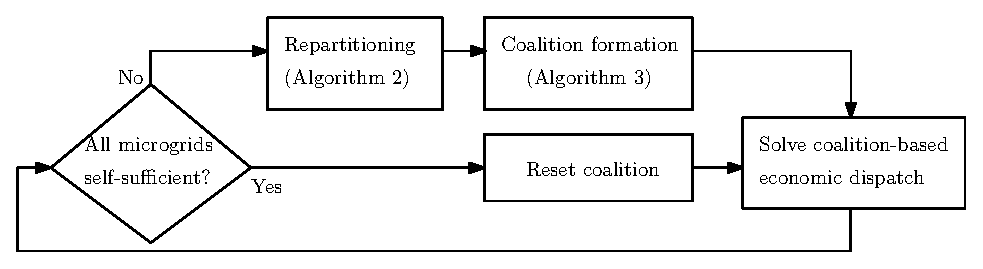
\includegraphics[scale=0.5]{img/ov_sch}
	\caption{The overall scheme of the proposed method.
	}
	\label{fig:prop_sch}
\end{figure}
%\fi
%\paragraph*{the goals} 


 
%\paragraph*{Reformulate the economic dispatch problem}
%In this regard, as shown in Proposition \ref{lem:net2mg},  Problem \eqref{eq:MPC_net} is reformulated as an economic dispatch problem of interconnected microgrids. 

\section{Event-triggered repartitioning scheme}
\label{sec:rep_sch}
Since the loads in the network vary over time, the network might need to be repartitioned to maintain the level of self-sufficiency. In this section, first we state the repartitioning problem. Afterward, we present the repartitioning process, which includes when and how the repartitioning must be performed. Furthermore, we also provide an analysis of the  repartitioning outcome.

\subsection{Repartitioning Problem Formulation}
Prior to presenting the methodology that we propose, we establish some definitions that will be used throughout the remainder of the paper. 

\begin{defn}[Non-overlapping partition]
	\label{def:nop}
	The set $\boldsymbol{\mathcal{M}}~=~\{\mathcal{M}_1, \mathcal{M}_2, \dots, \mathcal{M}_m \}$ defines $m$ non-overlapping partitions of graph $\mathcal{G}=(\mathcal{N},\mathcal{E})$ if $\bigcup_{p=1}^m \mathcal{M}_p = \mathcal{N}$ and $\mathcal{M}_p \cap \mathcal{M}_q = \emptyset$, for any $\mathcal{M}_p,\mathcal{M}_q \in \boldsymbol{\mathcal{M}}$ and $p \neq q$. %\eod
\end{defn}

\begin{defn}[Local imbalance]
	The local power imbalance of a subset of nodes $\mathcal{M}\subseteq\mathcal{N}$ at any $k\geq0$, denoted by $\Delta_{\mathcal{M},k}^{\mathrm{im}}$, is defined as
	\begin{equation}
		\Delta_{\mathcal{M},k}^{\mathrm{im}}= \sum_{i \in \mathcal{M}} \left(-\bar{u}_{i}^{\mathrm{g}} + {d}_{i,k}\right),
		\label{eq:p_im}
	\end{equation}
	where $\bar{u}_{i}^{\mathrm{g}}$ denotes the maximum capacity of dispatchable generation units, whereas ${d}_{i,k}$ follow \eqref{eq:ul} and the worst case disturbance, which is shown in \eqref{eq:w_ul}, is considered. \eod
	\label{def:local_imb}
\end{defn} 

%In the view of Definition \ref{def:local_imb}, the local imbalance of microgrid $\mathcal{M}_{p,k}$ indicates the difference between the aggregated worst-case load of microgrid $\mathcal{M}_{p,k}$ and the local power generation of microgrid $\mathcal{M}_{p,k}$. Based on Definition \ref{def:local_imb}, we define the self-sufficiency feature.
\begin{defn}[Self-sufficiency]
	A subset of nodes $\mathcal{M}\subseteq\mathcal{N}$ at any $k\geq0$ is self-sufficient if it has non-positive local imbalance at any step along the prediction horizon $h$, i.e., $\Delta_{\mathcal{M},\ell}^{\mathrm{im}} \leq 0,$ for all $\ell \in \{k,k+1,\dots,k+h-1 \}$. \eod
	\label{def:ss_mg}
\end{defn}
%begin{remark}
%Self-sufficiency  is suitably defined with the considered economic dispatch problem, which has a certain time horizon $h$. Furthermore, Definition \ref{def:ss_mg} will be used as the criterion to decide whether a repartitioning process is necessary at time instant $k$. 
%\end{remark}
%Moreover, we also define the imbalance and efficiency costs, which will be considered in the repartitioning problem.
%The imbalance cost \eqref{eq:j_im} penalizes a microgrid that does not have enough local power resource to meet the loads over the whole prediction horizon. On the other hand, we also consider another objective, namely the efficiency of each microgrid, which is provided in the following definition.
\begin{defn}[Imbalance cost]
	The imbalance cost of microgrid $\mathcal{M}_{p,k}\in\bm{\mathcal{M}}_k$ at any $k\geq0$, denoted by $J_{p,k}^{\mathrm{im}}$, is defined as
%	\begin{equation}
$	J_{p,k}^{\mathrm{im}} = \sum_{\ell =k}^{k+h-1}\max \left(0,\Delta_{\mathcal{M}_{p,k},\ell}^{\mathrm{im}}\right),$
%	\label{eq:j_im}
%	\end{equation}
	where $\Delta_{\mathcal{M}_{p,k},\ell}^{\mathrm{im}}$ is defined based on \eqref{eq:p_im}. \eod
	\label{def:im_cost}
\end{defn}
%Note that $c_{i}^{\mathrm{et}}$ can be set quite large to incentivize the decoupling among the microgrids.% Moreover, as can be seen in Definition \ref{def:eff_cost}, in order to compute $J_{p,k}^{\mathrm{ef}}$, the local controller must solve a local economic dispatch problem over $\tau+h$ time instants, which is derived from \eqref{eq:MPC_mg}.
\begin{defn}[Efficiency cost]
	\label{def:eff_cost}
	The efficiency cost of microgrid $\mathcal{M}_{p,k}\in\bm{\mathcal{M}}_k$ at any $k\geq0$, is defined  as follows:
	\begin{equation*}
	\begin{aligned}
	J_{p,k}^{\mathrm{ef}}=&\min_{\{\{\bm{u}_{i,\ell}\}_{i \in \mathcal{M}_{p,k}}\}_{\ell=k}^{k+h-1}} \sum_{\ell =k}^{k+h-1} \left(J_{p,\ell}^{\mu} + J_{p,\ell}^{{\epsilon}}\right)\\
	& \ \quad \mathrm{s.t.} \
	(\bm{u}_{i,\ell},\bm{v}_{i,\ell}) \in \mathcal{P}_i, \ \forall i \in \mathcal{M}_{p,k}, \\
	& \quad \quad v_{i,\ell}^j + v_{j,\ell}^i = 0, \ \forall j\in\mathcal{N}_i\cap\mathcal{M}_{p,k}, \ \forall i \in \mathcal{M}_{p,k},\\ 
	& \quad \quad \forall\ell \in\{k,\dots, k+h-1 \},
	\end{aligned}
	%\label{eq:j_ef}
	\end{equation*}
	where $J_{p,\ell}^{{\epsilon}}$ adds extra cost on the power transferred between one microgrid to another in order to minimize the dependency on the neighbors and is defined by
	%\begin{equation}
	$J_{p,\ell}^{{\epsilon}} = \sum_{i\in \mathcal{M}_{p,k}^{\mathrm{c}}} \sum_{j \in \mathcal{N}_i\backslash\mathcal{M}_{p,k}} c_{i}^{\mathrm{et}}(p_{ij,\ell}^{\mathrm{t}})^2,$
%	\label{eq:J_eps}
%	\end{equation}
	where $c_{i}^{\mathrm{et}} \in \mathbb{R}_{\geq 0}$ is the extra per-unit cost of transferring power.\eod
\end{defn}

Now, we state the repartitioning problem that will be solved supposing that the network is triggered to perform the repartitioning. 
First, assume that the network is initially partitioned into $m$ non-overlapping microgrids and denote the set of initial partition at $k=0$ by $\boldsymbol{\mathcal{M}}_0~=~\{\mathcal{M}_{1,0}, \mathcal{M}_{2,0}, \dots, \mathcal{M}_{m,0} \}$. 
\iffalse 
\begin{equation}
J^{\pi}(\mathcal{M}_{p,k})= \alpha_{\mathrm{im}} J_{p,k}^{\mathrm{im}} + \alpha_{\mathrm{ef}} J_{p,k}^{\mathrm{ef}}, 
\label{eq:j_pi}
\end{equation}
where $J_{p,k}^{\mathrm{im}}$ denotes the imbalance cost and $J_{p,k}^{\mathrm{ef}}$ denotes the efficiency cost, whereas $\alpha_{\mathrm{im}}$ and $\alpha_{\mathrm{ef}}$ denote the positive weight of these two cost components and can be regarded as tuning parameters of the repartitioning procedure. The imbalance cost is defined as follows:
\begin{equation}
J_{p,k}^{\mathrm{im}} = \sum_{\ell =k}^{k+\tau-1}\max \left(0,\sum_{i \in \mathcal{M}_{p,k}}p_{i,\ell}^{\mathrm{li}}\right),
\label{eq:j_im}
\end{equation}
where $p_{i,\ell}^{\mathrm{li}}$, which denotes the local power imbalance of bus $i$, is expressed as
\begin{equation}
p_{i,\ell}^{\mathrm{li}}=  \sum_{\tau =k}^{\ell} p_{i,\tau}^{\mathrm{li}}-\bar{p}_{i}^{\mathrm{g}}  - {p}^{\mathrm{re}}_{i,\tau} + {p}^{\mathrm{l}}_{i,\tau},
\label{eq:p_li}
\end{equation}
in which
${p}^{\mathrm{re}}_{i,\tau}$ and ${p}^{\mathrm{l}}_{i,\tau}$ follow \eqref{eq:ul} and \eqref{eq:re}, respectively, and the worst case disturbances, which are shown in \eqref{eq:ws_d}, are considered to robustify the solution against the uncertainties.  The imbalance cost \eqref{eq:j_im} penalizes a microgrid that does not have enough local power resource to meet the loads. Moreover, the efficiency cost is defined  as follows:
\begin{equation}
\begin{aligned}
J_{p,k}^{\mathrm{ef}}=&\min_{\{\{\bm{u}_{i,\ell}\}_{i \in \mathcal{M}_{p,k}}\}_{\ell=k}^{k+\tau+h-1}} \sum_{\ell =k}^{k+\tau+h-1} \left(J_{p,\ell}^{\mu} + J_{p,\ell}^{{\epsilon}}\right)\\
& \quad \quad \text{s. t. \eqref{eq:mg_loc_cons}-\eqref{eq:mg_loc_cons2}}, \forall\ell \in\{k,\dots, k+\tau+h-1 \},
\end{aligned}
\label{eq:j_ef}
\end{equation}
where $J_{p,\ell}^{{\epsilon}}$ adds extra cost on the power transferred between one microgrid to another in order to minimize the dependency on the neighbors and is defined as follows:
\begin{equation}
J_{p,\ell}^{{\epsilon}} = \sum_{i\in \mathcal{M}_{p,k}^{\mathrm{c}}} \sum_{j \in \mathcal{N}_i\backslash\mathcal{M}_{p,k}} c_{i}^{\mathrm{et}}(p_{ij,\ell}^{\mathrm{t}})^2,
\label{eq:J_eps}
\end{equation}
where $c_{i}^{\mathrm{et}}$ is the extra per-unit cost of transferring power and can be set quite large to minimize the usage of transferred power. As can be seen in \eqref{eq:j_ef}, in order to compute $J_{p,k}^{\mathrm{ef}}$, the local controller must solve a local economic dispatch problem over $\tau+h$ time instants, which is derived from \eqref{eq:MPC_mg}.  
\fi
Thus, for some time instants, at which the system must perform repartitioning,  the optimization problem that   must be solved is stated as follows: 
\begin{equation}
	\begin{aligned}
	&\min_{\boldsymbol{\mathcal{M}}_k}  \ \sum_{p=1}^m J^{\pi}(\mathcal{M}_{p,k})\\
	& \text{s.t. } \boldsymbol{\mathcal{M}}^{(0)}_k = \boldsymbol{\mathcal{M}}_{k-1},\\
	& \mathcal{M}_{p,k} \in \boldsymbol{\mathcal{M}}_k \text{ is non-overlapping and connected}.%
	\end{aligned}
	\label{eq:part_prob}%
\end{equation}
The cost function $J^{\pi}(\mathcal{M}_{p,k})$ is defined by 
\begin{equation}
J^{\pi}(\mathcal{M}_{p,k})= \alpha J_{p,k}^{\mathrm{im}} + J_{p,k}^{\mathrm{ef}}, 
\label{eq:j_pi}
\end{equation}
where $\alpha$ is the tuning parameter to determine the trade-off between both imbalance and efficiency costs. % Moreover, 
%$\mathcal{G}_{p,k}=(\mathcal{M}_{p,k},\mathcal{E}_{p,k} )$ denotes the subgraph of microgrid $\mathcal{M}_{p,k}$, with the set of edges denoted by $\mathcal{E}_{p,k}=\{(i,j)\in \mathcal{E}: i,j \in \mathcal{M}_{p,k} \}$ and $\lambda_2(L(\mathcal{G}_{p,k}))$ denotes the second smallest eigenvalue of the Laplacian matrix of subgraph $\mathcal{G}_{p,k}$. Equation \eqref{eq:con_mg} implies 
Moreover, each microgrid must be connected, i.e., the subgraph formed by each microgrid is connected. This constraint is imposed to avoid decoupling among the nodes within each microgrid. 
Furthermore, $\boldsymbol{\mathcal{M}}^{(0)}_k$ denotes the initial partition at time step $k$, which is equal to the partition at the previous time step, $k-1$. %In particular, for $k=\tau$, $\boldsymbol{\mathcal{M}}^{(0)}_k = \boldsymbol{\mathcal{M}}_0$.  
In addition, Assumption \ref{as:in_par}, which is related to the initial partition $\boldsymbol{\mathcal{M}}_0$, is considered.
\begin{assum}
	\label{as:in_par}
	The initial partition $\boldsymbol{\mathcal{M}}_0$ is non-overlapping with connected microgrids. %\eod 
\end{assum}
%\begin{rem}
%	The initial partition $\boldsymbol{\mathcal{M}}_0$ can be obtained by solving an optimal microgrid construction problem \cite{barani2018,arefifar2012}. %Moreover, any graph-partitioning methods, such as \cite{ocampo2011}, can be implemented to obtain an initial partition $\boldsymbol{\mathcal{M}}_0$ and the proposed repartitioning process can also be carried out at $k=0$ to refine the initial partition. 
	%\eod
%\end{rem}


\subsection{Repartitioning Process}

The repartitioning process consists of two main steps. The first step is to determine whether the system must perform the repartitioning and the second step is to actually perform the repartitioning. The event that triggers a repartitioning process is the existence of a microgrid that is not self-sufficient (c.f. Definition \ref{def:ss_mg}). In this regard, the triggering mechanism is provided in Algorithm \ref{alg:trig}. 
\begin{alg}[Triggering mechanism]
	\label{alg:trig}
	  \hfill
	\begin{enumerate}
		\item For each microgrid $\mathcal{M}_{p,k-1} \in\boldsymbol{\mathcal{M}}_{k-1}$, evaluate its self-sufficiency at $k$, based on Definition \ref{def:ss_mg}.
		\item If a microgrid is not self-sufficient, raise a flag to start repartitioning procedure. Otherwise wait until all microgrids perform step 1.
		\item If the flag to start the repartitioning procedure is not raised, then keep the  current partition, i.e., $\boldsymbol{\mathcal{M}}_{k}=\boldsymbol{\mathcal{M}}_{k-1}$. \eod
	\end{enumerate}
\end{alg}
%At each time instant $k$, first the controllers in the network execute Algorithm \ref{alg:trig}. Furthermore, when the flag to perform repartitioning is raised, we assume that all other microgrids can receive this information. This assumption can be fulfilled if the controllers have an either all-to-all communication network or at least a connected communication network.% When the communication network of the microgrids is connected, there exists a path from a microgrid to any other microgrid that can be used to relay this information.

Now, we discuss the repartitioning process, where the controllers cooperatively solve Problem \eqref{eq:part_prob}. We propose an iterative local improvement algorithm that can be performed in a distributed and synchronous manner. %The main idea of the algorithm is as follows. At each iteration, one node (bus) is proposed to be moved from one microgrid to a neighboring microgrid in order to improve the total cost. Therefore, 
Consider the initial partition $\boldsymbol{\mathcal{M}}_k^{(0)}$. Moreover, denote the iteration number by superscript $(r)$ and the set of boundary busses of microgrid $\mathcal{M}_{p,k}$, i.e., busses that are connected (coupled) to at least one bus that belongs to another microgrid by $\mathcal{M}_{p,k}^{\mathrm{c}}=\{i: (i,j) \in \mathcal{E}, i\in \mathcal{M}_{p,k}, j\in \mathcal{N}\backslash\mathcal{M}_{p,k} \}$. Then, the repartitioning procedure is stated in Algorithm \ref{alg:repartitioning}. %\color{blue}
Note that Algorithm \ref{alg:repartitioning} can be stopped when it reaches a predefined maximum  number of iteration $\bar{r}$.  \color{black}

\begin{alg}[Repartitioning procedure]
	\label{alg:repartitioning}
	Suppose that microgrid $\mathcal{M}_{p,k}$ is chosen to propose a node that will be moved at the $r^{\text{th}}$ iteration. Then, the steps at each iteration are described below:
	
	\begin{enumerate}
		\item Microgrid $\mathcal{M}_{p,k}$ computes $J^{\pi}(\mathcal{M}_{p,k}^{(r)})$, which is the local cost function at the $r^{\text{th}}$ iteration, based on \eqref{eq:j_pi}.
		\item Microgrid $\mathcal{M}_{p,k}$ computes a node that will be offered to be moved, denoted by $\theta_p$, as follows:
		\begin{equation}
		\theta_p \in \arg\min_{\theta \in \mathcal{M}_{p,k}^{\theta(r)}} J^{\pi}(\mathcal{M}_{p,k}^{(r)}\backslash\{\theta \}),
		\label{eq:theta_p}
		\end{equation}
		where $\mathcal{M}_{p,k}^{\theta(r)} \subseteq \mathcal{M}_{p,k}^{\mathrm{c}(r)}$ is a subset of boundary busses that do not disconnect microgrid $\mathcal{M}_{p,k}$ when removed, i.e., the graph form by $\mathcal{M}_{p,k}^{(r)} \backslash \{\theta \}$, for $\theta \in \mathcal{M}_{p,k}^{\theta(r)}$, is connected. The node   $\theta_p$ is randomly selected from the set of minimizers of \eqref{eq:theta_p}.
		\item %If the set of minimizers is empty, then the algorithm jumps to the next iteration. Otherwise, 
		Microgrid $\mathcal{M}_{p,k}$ computes the local cost difference if $\theta_p$ is moved out from microgrid $\mathcal{M}_{p,k}$, i.e.,
		\begin{equation}
		\Delta J^{\pi(r)}_p = J^{\pi}(\mathcal{M}_{p,k}^{(r)}\backslash\{\theta_p \}) - J^{\pi}(\mathcal{M}_{p,k}^{(r)}).
		\label{eq:delta_Jp}
		\end{equation} 
		\item Microgrid $\mathcal{M}_{p,k}$ shares the information of $\theta_p$ and $\Delta J^{\pi(r)}_p$ to the related neighboring microgrids $\mathcal{M}_{q,k}^{(r)} \in \mathcal{N}_{\theta_p}'=
		\{\mathcal{M}_{q,k}^{(r)}: (\theta_p,j) \in \mathcal{E}, j \in \mathcal{M}_{q,k}^{(r)} \}$.
		\item  All neighbors $\mathcal{M}_{q,k}^{(r)} \in \mathcal{N}_{\theta_p}'$ compute the expected total cost difference if $\theta_p$ is moved from microgrid $\mathcal{M}_{p,k}^{(r)}$ to microgrid $\mathcal{M}_{q,k}^{(r)}$, as follows:
		\begin{equation}
		\Delta J^{\pi(r)}_{\mathrm{t},q} = J^{\pi}(\mathcal{M}_{q,k}^{(r)}\cup\{\theta_p \}) - J^{\pi}(\mathcal{M}_{q,k}^{(r)})+\Delta J^{\pi(r)}_p,
		\label{eq:delta_Jq}
		\end{equation}
		and send the information of $\Delta J^{\pi(r)}_{\mathrm{t},q}$ to microgrid $\mathcal{M}_{p,k}$.
		\item Microgrid $\mathcal{M}_{p,k}$ selects the neighbor that will receive $\theta_p$ as follows:
		%\begin{equation}
		$q^{\star} \in \arg\min_{q \in \mathcal{N}_{\theta_p}'}\Delta J^{\pi(r)}_{\mathrm{t},q},
		$%\end{equation}
		where $q^{\star}$ is randomly chosen from the set of minimizers.
		\item  If $\Delta J^{\pi(r)}_{\mathrm{t},q^{\star}} \leq 0$, then the partition is updated as follows:
		%\begin{align}
		$\mathcal{M}_{p,k}^{(r+1)} = \mathcal{M}_{p,k}^{(r)}\backslash \{\theta_p\},\
		\mathcal{M}_{q^{\star},k}^{(r+1)} = \mathcal{M}_{q^{\star},k}^{(r)}\cup \{\theta_p\}.
		$ %\end{align}
		Otherwise, the algorithm jumps to the next iteration, $r+1$. \eod
	\end{enumerate}
\end{alg}


%The repartitioning procedure can be stopped when it reaches a predefined maximum  number of iteration $\bar{r}$. 
%Proposition \ref{prop:sol_alg} characterizes the solution obtained by the proposed algorithm.  
%\vspace{-8pt} 
\begin{prop}
	\label{prop:sol_alg}
	Let $\boldsymbol{\mathcal{M}}_0$ be the initial partition at $k=0$ and Assumption \ref{as:in_par} hold. At any time instant at which the repartitioning process is triggered, the output of Algorithm \ref{alg:repartitioning} is a non-overlapping partition with connected microgrids and converges to a local minimum. \eod 
\end{prop}
%\vspace{-12pt} 



\begin{pf*}{Proof.}
	Define by $\kappa$ the time instant at which the repartitioning process is triggered, i.e., there exists at least one microgrid in $\boldsymbol{\mathcal{M}}_{\kappa}$ that is not self-sufficient. Let $\kappa_0$ be the first (smallest) repartitioning instant. Notice that the initial partition $\boldsymbol{\mathcal{M}}^{(0)}_{\kappa}$, at any repartitioning instant $\kappa > \kappa_0$, equals to the solution of Algorithm \ref{alg:repartitioning} at the previous repartitioning instant. Therefore, if at $\kappa_0$ the assertion holds, then it also holds for any repartitioning instants. Hence, now we only need to evaluate the outcome of the repartitioning process at $\kappa_0$. 
	Since the system is not repartitioned when $k<\kappa_0$, the initial partition at $\kappa_0$, $\boldsymbol{\mathcal{M}}^{(0)}_{\kappa_0}=\boldsymbol{\mathcal{M}}_0$, is non-overlapping with connected microgrids due to Assumption \ref{as:in_par}. Moreover, at any iteration of the repartitioning procedure, the node proposed to be moved is selected from $\mathcal{M}_{p,{\kappa_0}}^{\theta (r)}$, which is the set of boundary nodes that do not cause the disconnection of the associated microgrid when removed (see \eqref{eq:theta_p}). At the end of the iteration, either one node is moved from one microgrid to another or no node is moved. These facts imply that, at the end of any iteration, $\boldsymbol{\mathcal{M}}^{(r)}_{\kappa_0}$ remains non-overlapping and the connectivity of each microgrid is maintained. 
	Now, we show the convergence of the repartitioning solution. To this end, let the total cost at the beginning of iteration $r$  be denoted by $J^{\pi(r)}_{\mathrm{t}} = \sum_{p=1}^m J^{\pi}(\mathcal{M}_{p,{\kappa}})$. The convergence is proved by showing that the evolution of the total cost is non-increasing. Suppose that $\theta_p$ is moved from microgrid $p$ to microgrid $q^{\star}$. Therefore, we have
	\vspace{-5pt}
	\begin{align*}
	J^{\pi(r+1)}_{\mathrm{t}}- J^{\pi(r)}_{\mathrm{t}} 
	&= J^{\pi}(\mathcal{M}_{p,k}^{(r+1)}) - J^{\pi}(\mathcal{M}_{p,{\kappa}}^{(r)}) \\& \quad + J^{\pi}(\mathcal{M}_{q^{\star},{\kappa}}^{(r+1)}) - J^{\pi}(\mathcal{M}_{q^{\star},{\kappa}}^{(r)})\\
	%&= J^{\pi}(\mathcal{M}_{p,{\kappa}}^{(r)}\backslash\{\theta_p \}) - J^{\pi}(\mathcal{M}_{p,{\kappa}}^{(r)}) \\ & \quad + J^{\pi}(\mathcal{M}_{q^{\star},{\kappa}}^{(r)}\cup\{\theta_p \}) - J^{\pi}(\mathcal{M}_{q^{\star},{\kappa}}^{(r)})\\
	%&= \Delta J^{\pi(r)}_p + J^{\pi}(\mathcal{M}_{q^{\star},{\kappa}}^{(r)}\cup\{\theta_p \}) - J^{\pi}(\mathcal{M}_{q^{\star},{\kappa}}^{(r)})\\
	&=\Delta J^{\pi(r)}_{\mathrm{t},q^{\star}} \leq 0.
	\end{align*}
	The first equality follows from the fact that only the local costs of microgrids $p$ and $q^{\star}$ change after iteration $r$. The second equality follows from \eqref{eq:delta_Jp} and \eqref{eq:delta_Jq}, and the inequality comes from the condition imposed in step 7 of Algorithm \ref{alg:repartitioning}, where $\theta_p$ is not moved if  $\Delta J^{\pi(r)}_{\mathrm{t},q^{\star}} > 0$. When no node is moved, $J^{\pi(r+1)}_{\mathrm{t}}- J^{\pi(r)}_{\mathrm{t}}=0$. \eod
\end{pf*}

%\begin{rem}
%	After the network is repartitioned by Algorithm \ref{alg:repartitioning}, not all microgrids might be self-sufficient. Note that in general, Problem \eqref{eq:MPC_net} might actually have feasible solutions that require high power exchange, implying it might be impossible to partition the network into self-sufficient microgrids.
%\end{rem}




\section{Coalition-based economic dispatch scheme}
\label{sec:nc_ed}
In this section, the non-centralized economic dispatch scheme based on the previously explained repartitioning approach is discussed. %The main objective of the scheme is to have as less communication traffic as possible. In this regard, 
We let each self-sufficient microgrid to solve its local economic dispatch problem and does not allow this microgrid to exchange power with its neighbors. Therefore, by imposing an additional constraint, self-sufficient microgrids do not need to communicate with its neighbors to dispatch its components. However, a fully decentralized method can only be performed if all microgrids are self-sufficient. For any microgrid that is not self-sufficient, its local economic dispatch problem might be infeasible since local power production is not enough to meet the load.  Since the repartitioning outcome does not guarantee the self-sufficiency of each microgrid, then the microgrids that are not self-sufficient form a coalition with some other microgrids such that the resulting economic dispatch problem that must be solved by each coalition is feasible. Note that in general, Problem \eqref{eq:MPC_net} might actually have feasible solutions that require high power exchange, implying it might be impossible to partition the network into self-sufficient microgrids.

\subsection{Coalition formation}
%\paragraph{why coalition is needed?}
%\paragraph{brief explanation about the main idea} how it works. Creating a coalition of self-sufficient microgrids.
%\paragraph{coalition} 
%We adapt the notion of coalition from coalitional control framework \cite{fele2017,fele2018}, in which only sub-systems that belong to the same coalition cooperatively compute their control inputs, whereas those that do not belong to the coalition can independently compute their control inputs. %In this regard, it means that Problem \eqref{eq:MPC_mg} will be decomposed into a number of subproblems, each of which will be solved by a coalition. The decomposition is possible due to the self-sufficiency and by adding extra constraints, as will be shown later in Section \ref{sec:nc_ed}.
In order to describe the coalition formation procedure, denote by $\mathcal{C}_{p,k}$ and $\mathcal{D}_{p,k}$ the set of nodes and the set of microgrids that belong to coalition $p$, respectively. We  assign one pair $(\mathcal{C}_{p,k},\mathcal{D}_{p,k})$ to each microgrid $\mathcal{M}_{p,k}$ to keep tracking the nodes and neighboring microgrids with which it forms a coalition. The coalition formation mechanism is described in Algorithm \ref{alg:clust}. 
\begin{alg}[Coalition formation procedure]
	\label{alg:clust}
	\hfill
	
	Each microgrid $\mathcal{M}_{p,k}$ defines $\mathcal{C}_{p,k}^{(0)}=\mathcal{M}_{p,k}$ and $\mathcal{D}_{p,k}^{(0)}=\{\mathcal{M}_{p,k}\}$. 
	While $r < m-1$, do:
	\begin{enumerate}
		
		\item Each microgrid $\mathcal{M}_{p,k}$ evaluates whether its coalition is self-sufficient based on Definition \ref{def:ss_mg}, i.e., whether $ \Delta_{\mathcal{C}_{p,k}^{(r)},\ell}^{\mathrm{im}} \leq 0, \quad \forall \ell \in \{k,\dots,k+h-1 \},$
		holds true. 
		\item If coalition $\mathcal{C}_{p,k}^{(r)}$ is self-sufficient, then microgrid $\mathcal{M}_{p,k}$ waits for commands until $r=m-1$.  
		\item Otherwise, microgrid $\mathcal{M}_{p,k}$ initiates a coalition merger by sending $\Delta_{\mathcal{C}_{p,k}^{(r)},\ell}^{\mathrm{im}}$, for all $\ell \in \{k,\dots,k+h-1 \}$, to the microgrids that do not belong to coalition $\mathcal{C}_{p,k}^{(r)}$ but they have physical connections with at least one bus in coalition $\mathcal{C}_{p,k}^{(r)}$, i.e.,  $\mathcal{M}_{q,k} \in \mathcal{N}_{p,k}^{\mathrm{c}}= \{\mathcal{M}_{q,k}: (i,j)\in \mathcal{E}, i \in \mathcal{C}_{p,k}^{(r)}, j \in \mathcal{M}_{q,k}, \mathcal{C}_{q,k}^{(r)} \neq \mathcal{C}_{p,k}^{(r)}  \}$. Note that if $\mathcal{N}_{p,k}^{\mathrm{c}}=\emptyset$, then $\mathcal{M}_{p,k}$ waits for commands until  $r=m-1$. \color{black}
		\item For each neighbor $\mathcal{M}_{q,k} \in \mathcal{N}_{p,k}^{\mathrm{c}}$, if it is not communicating with another microgrid, then it computes 
		$J_{q}^{\mathrm{cim}}= \sum_{\ell =k}^{k+h-1} \max\left(0,\Delta_{\mathcal{C}_{q,k}^{(r)},\ell}^{\mathrm{im}}+\Delta_{\mathcal{C}_{p,k}^{(r)},\ell}^{\mathrm{im}}\right).$ Otherwise, $J_{q}^{\mathrm{cim}}=\infty$. Then, it sends back $J_{q}^{\mathrm{cim}}$ to coalition $\mathcal{C}_{p,k}^{(r)}$.  
		\item Based on $J_{q}^{\mathrm{cim}}$, microgrid $\mathcal{M}_{p,k}$ chooses the neighbor that it will merge with as a coalition, as follows: 
		\begin{equation*}
		q^{\star}\in\arg\min_{\mathcal{M}_{q,k} \in \mathcal{N}_{p,k}^{\mathrm{c}}} J_{q}^{\mathrm{cim}} \quad \mathrm{s.t.} \ J_{q}^{\mathrm{cim}} < \infty.
		\end{equation*}
		\item Update the coalition sets, i.e.,  $\mathcal{C}_{\rho,k}^{(r+1)} = \mathcal{C}_{\rho,k}^{(r)}\cup \mathcal{C}_{q^{\star},k}^{(r)}$ and $\mathcal{D}_{\rho,k}^{(r+1)} = \mathcal{D}_{\rho,k}^{(r)} \cup \mathcal{D}_{q^{\star},k}^{(r)}$, for all $\mathcal{M}_{\rho,k}\in\mathcal{D}_{p,k}^{(r)}$ and $\mathcal{C}_{\rho,k}^{(r+1)} = \mathcal{C}_{\rho,k}^{(r)}\cup \mathcal{C}_{p,k}^{(r)}$ and $\mathcal{D}_{\rho,k}^{(r+1)} = \mathcal{D}_{\rho,k}^{(r)} \cup \mathcal{D}_{p,k}^{(r)}$, for all $\mathcal{M}_{\rho,k}\in\mathcal{D}_{q^{\star},k}^{(r)}$.%, and $\mathcal{C}_{q^{\star},k}^{(r+1)}= \mathcal{C}_{p,k}^{(r)}\cup \mathcal{C}_{q^{\star},k}^{(r)}$. 
		\item $r\leftarrow r+1$ and go back to step 1. %\eod
	\end{enumerate}
\end{alg}
%The outcome of Algorithm \ref{alg:clust} is stated as follows.
\begin{prop}
	\label{prop:alg_clus}
	By performing Algorithm \ref{alg:clust}, either all resulting coalitions $\mathcal{C}_{p,k}^{(m-1)}$, for $p=1,\dots,m$, are self-sufficient or all coalitions are merged, i.e., $\mathcal{C}_{p,k}^{(m-1)}=\mathcal{N}$, for $p=1,\dots,m$. \eod
\end{prop}

%\vspace{-18pt}
%\iffalse

\begin{pf*}{Proof.}
	%If all microgrids  $\mathcal{M}_{p,k} \in\boldsymbol{\mathcal{M}}_k$ are self-sufficient, then $\mathcal{C}_{p,k}^{(0)}$, for all $p=1,\dots,m$, are self-sufficient. Therefore, $\mathcal{C}_{p,k}^{(r)}=\mathcal{C}_{p,k}^{(0)}$, for any $r\geq1$. Now, we consider the case when there exists at least one microgrid in $\boldsymbol{\mathcal{M}}_k$ that is not self-sufficient. According to the algorithm, at least one coalition that is not self-sufficient is merged with its neighboring coalition per iteration. If at the end of an iteration all coalitions are self-sufficient, then at the Since the number of initial coalitions is finite, i.e., $m$, then there exists a finite number of iterations must be performed such that all coalitions are merged $\mathcal{C}_{p,k}=\mathcal{N}$
	 %Firstly, notice that the number of iterations $(r)$ is upper-bounded by $m$. 
	 %If all microgrids  $\mathcal{M}_{p,k} \in\boldsymbol{\mathcal{M}}_k$ are self-sufficient, then $\mathcal{C}_{p,k}^{(0)}$, for all $p=1,\dots,m$, are self-sufficient. As stated in step 2, all microgrids keep the initial coalitions, i.e.,   $\mathcal{C}_{p,k}^{(m)}=\mathcal{C}_{p,k}^{(0)}$, for all $p=1,\dots,m$. Now, we consider that there exists at least one microgrid in $\boldsymbol{\mathcal{M}}_k$  that is not self-sufficient. Equivalently, there exists at least one coalition  $\mathcal{C}_{p,k}^{(0)}$ that is not self-sufficient. 
	 At each iteration $r<m-1$, the evaluation in step 1 has two mutually exclusive outcomes:
	 %\vspace{-10pt}
	 \begin{enumerate}
	 		 	\setlength\itemsep{0.0em}
	 	\item All coalitions are self-sufficient.
	 	\item There exist some coalitions that are not self-sufficient.
	 \end{enumerate}
% \vspace{-10pt} 
	 In case 1, we have that $\mathcal{C}_{p,k}^{(m-1)}=\mathcal{C}_{p,k}^{(r)}$, for all $p=1,\dots,m$ since the coalitions do not change from the $r^{\mathrm{th}}$ iteration until the $(m-1)^{\mathrm{th}}$ iteration.  Note that when all microgrids  $\mathcal{M}_{p,k} \in\boldsymbol{\mathcal{M}}_k$ are self-sufficient, then $\mathcal{C}_{p,k}^{(0)}$, for all $p=1,\dots,m$, are self-sufficient. Therefore, this case is also included here. 
	 In case 2, according to steps 3-6, at least one of the coalitions that are not self-sufficient will be merged with one of its neighboring coalitions at the next iteration $r+1$. Since the number of initial coalitions is finite ($m$), then if case 2 keeps occurring, all coalitions will be merged, i.e., $\mathcal{C}_{p,k}=\mathcal{N}$, for all $p=1,\dots,m$, at a finite number of iterations. Otherwise, case 1 will occur. Furthermore, in case 2, the minimum number of coalitions that can perform steps 3-6 (merging with one of its neighboring coalitions) is one. If, for $r\geq1$, only one coalition merges with one of its neighbors, then it requires $m-1$ iterations to merge all coalitions. %Note that if more than one pair of coalitions merges at least in one iteration, then the number of iterations required to merge all of them is less than $m-1$.
	  \eod \color{black}
\end{pf*}
% \fi
%\begin{rem}
%	Notice that in steps 3-6 more than one coalition that is not self-sufficient can initiate a coalition merger. However, in step 4, each coalition can only be asked by one neighbor at each iteration. In this regard, step 4 can be executed by the principle of first comes first served. %\eod
%\end{rem}

\subsection{Non-centralized economic dispatch}
In this section, we outline the proposed scheme to solve Problem \eqref{eq:MPC_net} based on the coalitions that have been formed. Note that when all microgrids $\mathcal{M}_{p,k}, \ p=1,\dots,m,$ are self-sufficient, the coalitions are reset as in the initialization of Algorithm \ref{alg:clust}, i.e., $\mathcal{C}_{p,k}=\mathcal{M}_{p,k}$, for $p=1,\dots,m$. First, we reformulate Problem \eqref{eq:MPC_net} as shown in Proposition \ref{lem:net2co}.
\begin{prop}
	\label{lem:net2co}
	Suppose that, at time instant $k$, the network is partitioned into $m$ non-overlapping microgrids, defined by the set $\boldsymbol{\mathcal{M}}_k~=~\{\mathcal{M}_{1,k}, \mathcal{M}_{2,k}, \dots, \mathcal{M}_{m,k} \}$. Furthermore, coalitions of microgrids, denoted by $\mathcal{C}_{p,k}$, for $p=1,\dots,m$, are formed based on Algorithm \ref{alg:clust}. 
	Then, Problem \eqref{eq:MPC_net} is equivalent to
	\begin{subequations}
		\begin{align}
		&\min_{\{\{(\bm{u}_{i,\ell},\bm{v}_{i,\ell})\}_{i \in \mathcal{N}}\}_{\ell=k}^{k+h-1}}  \sum_{p=1}^{m} \sum_{i \in \mathcal{M}_{p,k}} \sum_{\ell =k}^{k+h-1}  J_{i,\ell}(\bm{u}_{i,\ell},\bm{v}_{i,\ell}) \label{eq:mg_cost_func}\\
		&\mathrm{s.t. }  
		\quad (\bm{u}_{i,\ell},\bm{v}_{i,\ell}) \in \mathcal{P}_i, \ \forall i \in \mathcal{C}_{p,k},  \label{eq:mg_loc_cons}\\
		&\qquad \quad v_{i,\ell}^j + v_{j,\ell}^i = 0, \ \forall j \in \mathcal{N}_i\cap\mathcal{C}_{p,k}, \  \forall i \in \mathcal{C}_{p,k},  \label{eq:mg_loc_cons2}\\
		&\qquad \quad v_{i,\ell}^j + v_{j,\ell}^i = 0, \ \forall j \in \mathcal{N}_i\backslash\mathcal{C}_{p,k}, \ \forall i \in \mathcal{C}_{p,k},  \label{eq:mg_coup_cons}
		\end{align}
		\label{eq:MPC_mg}%
	\end{subequations}
	for all $\mathcal{C}_{p,k}$, where $p=1,\dots,m$, and all $\ell \in\{k,\dots, k+h-1 \}$. \eod %$J_{p,\ell}^{\mu}$ in the cost function \eqref{eq:mg_cost_func} is defined as follows 
	%\begin{equation}
	%\eod%\end{equation}
\end{prop}
%\iffalse

\begin{pf*}{Proof.}
	Since $\mathcal{M}_{p,k}$, for each $p=1,\dots,m$, is non-overlapping, the cost function \eqref{eq:net_cost_func} is equal to  \eqref{eq:mg_cost_func}. Moreover, since $\bigcup_{p=1}^m \mathcal{C}_{p,k} = \mathcal{N}$,  \eqref{eq:net_loc_cons} is equivalent to \eqref{eq:mg_loc_cons}. Furthermore, \eqref{eq:net_coup_cons} is decomposed into \eqref{eq:mg_loc_cons2} and \eqref{eq:mg_coup_cons}.  \eod
\end{pf*}
%\fi
\begin{rem}
	\label{rem:const_coal}
	For each coalition $\mathcal{C}_{p,k}$, \eqref{eq:mg_loc_cons} and \eqref{eq:mg_loc_cons2} are local constraints. Particularly for the constraints in \eqref{eq:mg_loc_cons2}, some of them might involve two different microgrids. Meanwhile, \eqref{eq:mg_coup_cons} are coupling constraints with other coalitions. \eod
\end{rem}
%Suppose that at the end of the coalition formation procedure there exist $c$ distinct coalitions whose elements are different from one to another, where $c\leq m$. Note that when $\mathcal{C}_{p,k}=\mathcal{C}_{q,k}$, microgrids $\mathcal{M}_{p,k}$ and $\mathcal{M}_{q,k}$ belong to the same coalition. 
%A non-centralized economic dispatch scheme will be formulated for these coalitions by decomposing Problem \eqref{eq:MPC_mg} such that each coalition solves its own economic dispatch. The decomposition is done by not allowing power exchange between two neighboring coalitions. 
By decomposing Problem \eqref{eq:MPC_mg}, we formulate the decentralized MPC-based economic dispatch problem that must be solved at each coalition $\mathcal{C}_{p,k}$, for $p=1,\dots,m$, as follows:
\begin{subequations}
	\begin{align}
	&\min_{\{\{(\bm{u}_{i,\ell},\bm{v}_{i,\ell})\}_{i \in \mathcal{C}_{p,k}}\}_{\ell=k}^{k+h-1}} \sum_{i \in \mathcal{C}_{p,k}} \sum_{\ell =k}^{k+h-1}  J_{i,\ell}(\bm{u}_{i,\ell},\bm{v}_{i,\ell})\\
	&\text{s.t. } \quad  (\bm{u}_{i,\ell},\bm{v}_{i,\ell}) \in \mathcal{P}_i,   \label{eq:co_loc_cons}\\
		&\qquad \quad v_{i,\ell}^j + v_{j,\ell}^i = 0, \ \forall j \in \mathcal{N}_i\cap\mathcal{C}_{p,k},   \label{eq:co_loc_cons2}\\
		&\qquad \quad v_{i,\ell}^j = 0, \ \forall j \in \mathcal{N}_i\backslash\mathcal{C}_{p,k},  \label{eq:coup_dec_const}
	\end{align}
	\label{eq:lo_mpc}%
\end{subequations}
for all $i \in \mathcal{C}_{p,k}$ and $\ell \in\{k,\dots, k+h-1 \}$. Note that if microgrids $\mathcal{M}_{p,k}$ and $\mathcal{M}_{q,k}$ belong to the same coalition, i.e., $\mathcal{C}_{p,k}=\mathcal{C}_{q,k}$,  then they must cooperatively solve the same problem in a distributed manner. Additionally, if $c=m$, then each microgrid is self-sufficient, implying a fully decentralized scheme (without communication) is applied to the network. On the other hand, if $c=1$, then a fully distributed scheme (with neighbor-to-neighbor communication) is applied to the network.

Now, we show that Problem \eqref{eq:lo_mpc}, for any coalition, has a solution. Furthermore, the solution to Problem \eqref{eq:lo_mpc} is also a feasible solution to the original problem \eqref{eq:MPC_net}.
\begin{prop}
	Suppose that Assumption \ref{as:feas_ED_cent} holds and let the coalitions $\mathcal{C}_{p,k}$, for $p=1,\dots,m$, are formed by using Algorithm \ref{alg:clust}. Then,  there exists a unique solution to Problem \eqref{eq:lo_mpc}, for each coalition $\mathcal{C}_{p,k}$, where \ $p \in \{1,\dots,m\}$.
	% \eod
\end{prop}
%\iffalse

\begin{pf*}{Proof.}
Since the cost function is strictly convex, the uniqueness of the solution is guaranteed provided that the feasible set is nonempty. Therefore, we only need to show that Problem \eqref{eq:lo_mpc}, for any $\mathcal{C}_{p,k}$, has a  non-empty feasible set. Consider the outcome of Algorithm \ref{alg:clust} (c.f. Proposition \ref{prop:alg_clus}). If Algorithm \ref{alg:clust} results in one coalition over the whole network, i.e., $\mathcal{C}_{p,k}=\mathcal{N}$, for $p=1,\dots,m$, then it implies that all microgrids must solve the centralized economic dispatch problem \eqref{eq:MPC_mg} cooperatively. Therefore, in this case, for any $\mathcal{C}_{p,k}$, Problem \eqref{eq:lo_mpc} is equal to Problem \eqref{eq:MPC_mg}. Due to Assumption \ref{as:feas_ED_cent}, feasible solutions to Problem \eqref{eq:MPC_mg} exist. Otherwise, Algorithm \ref{alg:clust} results in at least two different self-sufficient coalitions. In this case, we have non-positive local imbalance (c.f. Definition \ref{def:local_imb}), i.e., the worst-case uncertain imbalance between loads and non-dispatchable generation can be met cooperatively by the distributed generation units within the coalition.  Therefore, there exists a non-empty subset of feasible solution of Problem \eqref{eq:MPC_mg} such that \eqref{eq:coup_dec_const}, for all $\mathcal{C}_{p,k}$, where $p=1,\dots,m$, hold, implying the existence of a non-empty feasible set of Problem \eqref{eq:lo_mpc}. \eod
\end{pf*}
%\fi 
\begin{prop}
	\label{prop:feas_of_orig}
	Let $(\bm{u}_{i,\ell}^{\star},\bm{v}_{i,\ell}^{\star})$, for all $\ell \in\{k,\dots, k+h-1 \}$ and $i\in\mathcal{C}_{p,k}$, be the solution to Problem \eqref{eq:lo_mpc}, for all coalitions  $\mathcal{C}_{p,k}$, where $p=1,\dots,m$. Then, they are also a feasible solution to Problem \eqref{eq:MPC_net}. %\eod
\end{prop}
%\iffalse

\begin{pf*}{Proof.}
	In Proposition \ref{lem:net2co}, we show that Problem \eqref{eq:MPC_mg} is equivalent with Problem \eqref{eq:MPC_net}, therefore we only need to show that $(\bm{u}_{i,\ell}^{\star},\bm{v}_{i,\ell}^{\star})$, for all $\ell \in\{k,\dots, k+h-1 \}$, $i\in\mathcal{C}_{p,k}$, and $p=1,\dots,m$, is a feasible solution to Problem \eqref{eq:MPC_mg}. Note that Problem \eqref{eq:lo_mpc} is obtained by decomposing Problem \eqref{eq:MPC_mg}.  As can be seen, the constraints \eqref{eq:mg_loc_cons}-\eqref{eq:mg_loc_cons2} are decomposed for each coalition and considered as \eqref{eq:co_loc_cons}-\eqref{eq:co_loc_cons2} in Problem \eqref{eq:lo_mpc}. Since $(\bm{u}_{i,\ell}^{\star},\bm{v}_{i,\ell}^{\star})$, for all $\ell \in\{k,\dots, k+h-1 \}$ and $i\in\mathcal{C}_{p,k}$, satisfy the constraints \eqref{eq:co_loc_cons}-\eqref{eq:co_loc_cons2}, they also satisfy \eqref{eq:mg_loc_cons}-\eqref{eq:mg_loc_cons2}. Finally, for any $\mathcal{C}_{p,k}$, by \eqref{eq:coup_dec_const}, we know that $v_{i,\ell}^{j\star}=v_{j,\ell}^{i\star}=0$, for all $j\in\mathcal{N}_i\backslash\mathcal{C}_{p,k}$, $i\in\mathcal{C}_{p,k}$, and $\ell\in\{k,\dots, k+h-1 \}$. From this fact, we obtain that $v_{i,\ell}^{j\star}+v_{j,\ell}^{i\star}=0$ for all $j\in\mathcal{N}_i\backslash\mathcal{C}_{p,k}$ $i\in\mathcal{C}_{p,k}$, and $\ell\in\{k,\dots, k+h-1 \}$, implying the satisfaction of the constraints in \eqref{eq:mg_coup_cons}. \eod
\end{pf*}
%\fi
%Finally, we note that the main issue in solving Problem \eqref{eq:lo_mpc} in a distributed way is the existence of coupling constraints among the microgrids in the same coalition, i.e.,
Finally, we note that due to the following coupling constraints,
\begin{equation}
v_{i,\ell}^j + v_{j,\ell}^i = 0, \quad \forall j \in \mathcal{N}_i\cap\mathcal{C}_{p,k}\backslash\mathcal{M}_{p,k}, \label{eq:coup_con_coal}
\end{equation}
for all  $\forall i \in \mathcal{C}_{p,k}$ and $\ell \in\{k,\dots, k+h-1 \}$ (c.f. Remark \ref{rem:const_coal}), a distributed Lagrangian approach, where the coupling constraints \eqref{eq:coup_con_coal} are relaxed, can be implemented to solve Problem \eqref{eq:lo_mpc}. In this regard, a distributed dual-ascent algorithm, such as that presented in \cite{ananduta2018}, can be applied to solve Problem \eqref{eq:lo_mpc}, in which more than one microgrid is involved. Note that, different distributed algorithms, e.g., \cite{boyd2011,wang2015,kraning2014,baker2016}, can also be chosen instead. Nevertheless, since there are available distributed algorithms in the literature that can be applied, we assume that the optimal solution to Problem \eqref{eq:lo_mpc} can be computed in a distributed manner.





\section{Sub-optimality and communication trade-off}
\label{sec:opt}
In this section, we discuss the sub-optimality and communication trade-off of the proposed scheme. 
%\subsection{Sub-optimality}
First, we show an estimation of the sub-optimality level achieved by the scheme. To that end, we state the collection of the optimization problems \eqref{eq:lo_mpc}, for all coalitions $\mathcal{C}_{p,k}, p=1,\dots,m$, as follows:
\begin{equation}
	\begin{aligned}
	&\min_{\{\{(\bm{u}_{i,\ell},\bm{v}_{i,\ell})\}_{i \in \mathcal{N}}\}_{\ell=k}^{k+h-1}} \sum_{i \in \mathcal{N}} \sum_{\ell =k}^{k+h-1}  J_{i,\ell}(\bm{u}_{i,\ell},\bm{v}_{i,\ell})\\
	&\text{s.t. \eqref{eq:co_loc_cons}, \eqref{eq:co_loc_cons2}, and \eqref{eq:coup_dec_const}, } \forall p \in \{1,\dots,m\},
	\end{aligned}
		\label{eq:lo_mpc_all}%
\end{equation}
for all $\ell \in\{k,\dots,k+h-1 \}$. Denote the optimal value of Problem \eqref{eq:lo_mpc_all} by $J^{\star}_k$. Note that $J^{\star}_k$ represents the cost function value of Problem \eqref{eq:MPC_net} computed by the proposed scheme. Furthermore, denote by $J_k^o$ the optimal value of Problem \eqref{eq:MPC_net} and define the sub-optimality measure as the difference between the cost function value computed using the proposed scheme and the optimal value of Problem \eqref{eq:MPC_net}, denoted by $\Delta J_k$, i.e., 
\begin{equation}
	\Delta J_k = J^{\star}_k-J^o_k. \label{eq:diff_J}
\end{equation}
%Therefore, an estimate of $\Delta J_k$ is shown in Proposition \ref{prop:est_difJ}.
\begin{prop}
	\label{prop:est_difJ}
	Let $J^{\star}_k$ and $J^o_k$ be the optimal values of Problems \eqref{eq:lo_mpc_all} and \eqref{eq:MPC_net} at time $k$, respectively. Furthermore, let $J^{b}_k$ denote the optimal value of the following optimization problem:
	\begin{equation}
	\begin{aligned}
	&\min_{\{\{(\bm{u}_{i,\ell},\bm{v}_{i,\ell})\}_{i \in \mathcal{N}}\}_{\ell=k}^{k+h-1}} \sum_{i \in \mathcal{N}} \sum_{\ell =k}^{k+h-1}  J_{i,\ell}(\bm{u}_{i,\ell},\bm{v}_{i,\ell})\\
	&\mathrm{s.t. } \text{ \eqref{eq:co_loc_cons} $\mathrm{and}$ \eqref{eq:co_loc_cons2} } \forall p \in \{1,\dots,m\}.
	\end{aligned}
	\label{eq:lb_mpc_all}%
	\end{equation}
	Then, the following estimate on the suboptimality measure $\Delta J_k$, defined in \eqref{eq:diff_J}, holds:
	\begin{equation}
		\Delta J_k \leq J^{\star}_k-J^b_k. \label{eq:est_diffJ}
	\end{equation}
\end{prop}
%\iffalse 
\begin{pf*}{Proof.}
	Note that Problem \eqref{eq:lb_mpc_all} can be obtained by relaxing Problem \eqref{eq:MPC_net}. In particular, the coupling constraint $v_{i,\ell}^j + v_{j,\ell}^i=0$, for each pair of nodes $i$ and $j$ that do not belong to the same coalition, is discarded in Problem \eqref{eq:lb_mpc_all}. Due to this relaxation, we can conclude that $J^b_k \leq J^o_k$. Moreover, based on Proposition \ref{prop:feas_of_orig}, the solution obtained by Problem \eqref{eq:lo_mpc}, for all coalitions $\mathcal{C}_{p,k}, \ p=1,\dots,m$, is also a feasible solution to Problem \eqref{eq:MPC_net}, implying that $J^o_k \leq J^{\star}_k$. Based on the preceding observations, the relation in \eqref{eq:est_diffJ} holds. \eod
\end{pf*}
%\fi
%\iffalse 
\begin{rem}
	\label{re:tight_bound}
	Consider the case when $\mathcal{C}_{p,k}=\mathcal{N}$, for $p=1,\dots,m$. In this case, for any $i\in \mathcal{N}$, all neighbors of node $i$, i.e., $j\in\mathcal{N}_i$, belong to the same coalition as that of node $i$. Thus, in \eqref{eq:coup_dec_const},  $\mathcal{N}_i\backslash\mathcal{C}_{p,k}=\emptyset$. This fact implies that Problem \eqref{eq:lo_mpc_all} is equivalent to Problem \eqref{eq:MPC_net} and Problem \eqref{eq:lb_mpc_all}, implying   $\Delta J_k=0$ and $J^{\star}_k-J^b_k=0$. Additionally, Problem \eqref{eq:lb_mpc_all} can be decomposed into {$m$ sub-problems, each of which can be assigned to each coalition}.\eod
\end{rem}
%\fi
%\begin{rem}
	%The optimal value of Problem \eqref{eq:lb_mpc_all} is a lower bound of Problem \eqref{eq:MPC_net}. Moreover, %Problem \eqref{eq:lo_mpc_all} is obtained from the coalition-based economic dispatch problem in \eqref{eq:lo_mpc} and Problem \eqref{eq:lb_mpc_all} is obtained from Problem \eqref{eq:lo_mpc_all}. Therefore, 
%	Problem \eqref{eq:lb_mpc_all} can also be decomposed into {$m$ sub-problems, each of which can be assigned to each coalition}.\eod %In particular, the sub-problem is as follows:
	%\begin{equation}
	%\begin{aligned}
	%&\min_{\{\{(\bm{u}_{i,\ell},\bm{v}_{i,\ell})\}_{i \in \mathcal{C}_{p,k}}\}_{\ell=k}^{k+h-1}} \sum_{i \in \mathcal{C}_{p,k}} \sum_{\ell =k}^{k+h-1}  J_{i,\ell}(\bm{u}_{i,\ell},\bm{v}_{i,\ell})\\
	%&\qquad \qquad \mathrm{s.t. } \text{ \eqref{eq:co_loc_cons} $\mathrm{and}$ \eqref{eq:co_loc_cons2}, }\forall \ell \in\{k,\dots,k+h-1 \}.
	%\end{aligned}
	%\label{eq:lb_mpc}%
%	\end{equation}
	%As mentioned in Remark \ref{re:tight_bound}, $\Delta J_k=J^{\star}_k-J^b_k=0$ when $\mathcal{C}_{p,k}=\mathcal{N}$, for $p=1,\dots,m$. Then, in this particular case, $J^b_k$ is not necessary to be computed. 
%\end{rem}

%\subsection{Communication cost}
%\color{red}
Now, we discuss the communication cost of the proposed scheme. Algorithms \ref{alg:repartitioning} and \ref{alg:clust} do require information exchange among the controllers. The total size of data exchanged throughout the process in Algorithms \ref{alg:repartitioning} and \ref{alg:clust} is $\mathcal{O}(m)$ per iteration. %It is obtained since, at each iteration, the microgrid selected to propose a node to be moved must send the information about the node, which is a scalar, to its neighbors and receives back the cost adjustment, which is also a scalar.  
%Furthermore, the total size of information exchanged in Algorithm \ref{alg:clust} is also $\mathcal{O}(m)$. %, since the information exchange process is similar to that of Algorithm \ref{alg:repartitioning}. 
Finally, we evaluate the size of data communicated when solving the coalition-based economic dispatch problem. Each coalition might need to use a distributed optimization method since there might be more than one microgrid in a coalition. As an example, we consider the dual-ascent algorithm \cite{ananduta2018} as the distributed optimization method. In this algorithm, the size of exchanged information is  $\mathcal{O}(m|\mathcal{N}|h)$ per iteration since each microgrid must exchange the coupled decision variables with each neighbor. 
In the best-case scenario, when all microgrids are self-sufficient, communication might not be necessary at all at one time instant. Furthermore, even if the repartitioning procedure is triggered, in the worst-case scenario, i.e., when the resulting coalition includes all microgrids, the extra amount of data must be exchanged to perform the repartitioning and coalition formation procedures is relatively much smaller than that of performing the distributed algorithm. In addition, for a coalition that has only one microgrid, its controller only needs to solve a local optimization problem once, which significantly reduces the computational burden as well.  
\color{black}

In comparison with existing methods that are based on distributed optimization algorithms, e.g., \cite{baker2016,wang2015,kraning2014,braun2016,guo2016}, the proposed scheme reduces the number of neighbors with which each agent must communicate since each agent only needs to communicate with a subset of neighbors that belong to the same coalition. This fact implies the reduction of communication flows. Moreover, the coalition-based problem \eqref{eq:lo_mpc} is relatively smaller than the network problem \eqref{eq:MPC_net}, thus intuitively a solution to \eqref{eq:lo_mpc} can be computed faster than a solution to \eqref{eq:MPC_net} using the same distributed iterative algorithm. 
%However, it is also important to note that when there exist at least two distinct coalitions, the solution obtained from the proposed scheme might be suboptimal. %As stated in Remark \ref{re:tight_bound}, we can only guarantee that the optimal solution is obtained when all controllers belong to the same coalition.% Additionally, distributed optimization methods, e.g. those that are proposed in \cite{baker2016,wang2015,kraning2014,braun2016,guo2016}, might also be implemented to solve the coalition-based problem \eqref{eq:lo_mpc}, for coalitions that consists of more than one agents/microgrids. 

%\color{red}
Finally, we discuss the practicality of performing the proposed scheme. As in any distributed scheme, local controllers must cooperate to perform the proposed method and a communication network must also be available. Since the partition of the electrical network is dynamic, a dynamic network, containing necessary communication links, might be required. Another possibility is by having an all-to-all network although in the process not all links will be used. Furthermore, each local controller must also be able to communicate with the active components of the network, i.e., the storage and dispatchable generation units. The second important note that we would like to mention that although in this paper we consider an MPC-based framework, where the set points are computed at each time instant, the proposed method can also be implemented for day-ahead economic dispatch without requiring any modification. In this case, the prediction horizon is set to be one day and prior to the computation of the decisions, the self-sufficiency of each microgrid is evaluated. \color{black}

\section{Case study}
\label{sec:case_st}
\begin{figure}
	\centering
	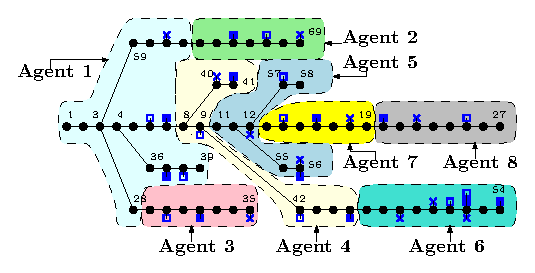
\includegraphics[scale=0.9]{img/top_sim1.eps}
	\caption{The topology of the PG\&E 69-bus distribution system and its 8-agent initial partition \cite{arefifar2012}. Squares indicate the distributed generation units, i.e., \textcolor{blue}{$\blacksquare$} and \textcolor{blue}{$\Box$} represent a renewable generation unit and a dispatchabale generator, respectively, whereas crosses, \textcolor{blue}{$\boldsymbol{\times}$}, indicate the storages.
	}
	\label{fig:cs_top}
\end{figure}
\iffalse 
\begin{table}
	\centering
	\caption{Parameters of the Network Components}
	\label{tab:param}
	\begin{tabular}{c c c c}
		\hline  \noalign{\smallskip}
		\textbf{Parameters} & \textbf{Value} & \textbf{Unit} & \textbf{Bus} \\ 
		\noalign{\smallskip}\hline  \noalign{\smallskip}
		$p^{\mathrm{g,min}}_i$, $p^{\mathrm{g,max}}_i$  & 0, 350 & kW  & $i \in \mathcal{N}^{\mathrm{dg}}$ \\ 		   
		\noalign{\smallskip}
		$x^{\mathrm{min}}_i$, $x^{\mathrm{max}}_i$, $x_{i,0}$ & 30, 100, 50  & \% & $i \in \mathcal{N}^{\mathrm{st}}$\\ 
		\noalign{\smallskip}
		$p^{\mathrm{ch}}_i$, $p^{\mathrm{dh}}_i$ & 100, 100 & kW & $i \in \mathcal{N}^{\mathrm{st}}$  \\ 
		\noalign{\smallskip}
		$e_{\mathrm{cap},i}$ & 1000 & kWh & $i \in \mathcal{N}^{\mathrm{st}}$   \\
		\noalign{\smallskip}
		$a_i$  & 1  & -   & $i \in \mathcal{N}^{\mathrm{st}}$\\
		\noalign{\smallskip}
		$c^{\mathrm{st}}_i$, $c^{\mathrm{g}}_i$  & 1, 10 & -  & $i \in \mathcal{N}$ \\
		\noalign{\smallskip}
		$c^{\mathrm{im}}_i$, $c^{\mathrm{t}}_i$ & 10, 1 & - & $i \in \mathcal{N}$ \\		
		\noalign{\smallskip}
		\hline
	\end{tabular}
\end{table}
\fi 
We consider the PG\&E 69-bus distribution network, as shown in Fig. \ref{fig:cs_top} where dispatchable, solar-based distributed generation, and storage units are added to the network. 
%Moreover,  the available load data are regarded as the maximum loads and the real load profiles and forecasts are generated based on the typical residential and commercial load profiles. The busses that have maximum load greater than 100 kW are considered to have a commercial load profile. Otherwise, they have a residential load profile. 
The simulation time is one day with the sampling time of 15 minutes, implying 96 time steps. Furthermore, the prediction horizon is set to be 8 time steps and the weight on the cost of the repartitioning problem is set as $\alpha=10^4$. %The other parameters of the network components are given in Table \ref{tab:param}. 

%\paragraph*{evolution of partitions formed}
%\paragraph*{evolution of coalitions formed}

The initial partition of the network is based on one of the partitioning results in \cite{arefifar2012}. How the microgrids form coalitions throughout the simulation can be seen in Figure \ref{fig:co_res}. %At $k=1,\dots,13$, all microgrids obtained from the initial partition of the network are still self-sufficient. Then, at $k=14$, for the first time the network must be repartitioned. Moreover, for $k=14,\dots,24$, the repartitioning and coalition formation procedures are always performed. During this period, two microgrids are not self-sufficient and join together as a coalition. At $k=25$, the repartitioning procedure produces self-sufficient microgrids, %as shown in Figure \ref{fig:part_res}.a, 
%and self-sufficiency is maintained until $k=57$. 
We can observe that 
 during the peak hours $57\leq k \leq 80$, coalitions must be formed and, even at a certain period, all microgrids must join as one coalition, whereas during the off-peak hours, self-sufficient microgrids can be formed. % We can also see gradual changes of the coalitions formed particularly at $k\geq57$. Moreover, towards the end of the simulation we can also see that by performing repartitioning of the network, the number of self-sufficient microgrids improves as the number of distinct coalitions also increases. Finally, at $k=96$, all the microgrids formed are self-sufficient, %as shown in Figure \ref{fig:part_res}.b. %In addition, one can compare the differences between the initial partition in Figure \ref{fig:cs_top} and the resulting partitions in Figure \ref{fig:part_res}.
%\paragraph*{suboptimality} 
Figure \ref{fig:deltaJ} shows the stage costs for all time steps and the sub-optimality of the proposed scheme. %As provided by Proposition \ref{prop:est_difJ}, the scheme might also compute an upper bound of the sub-optimality, which is shown by the dashed line in the bottom plot of Figure \ref{fig:deltaJ}. %The average sub-optimality throughout the simulation is $21.93\%$, whereas the average upper bound of the sub-optimality defined in Proposition \ref{prop:est_difJ} is $51.38\%$. %Furthermore, during $k=62,\dots,72$, when all microgrids form one coalition, the optimal cost values are obtained since a fully distributed scheme is employed.
\color{black}

\begin{figure}
	\centering
	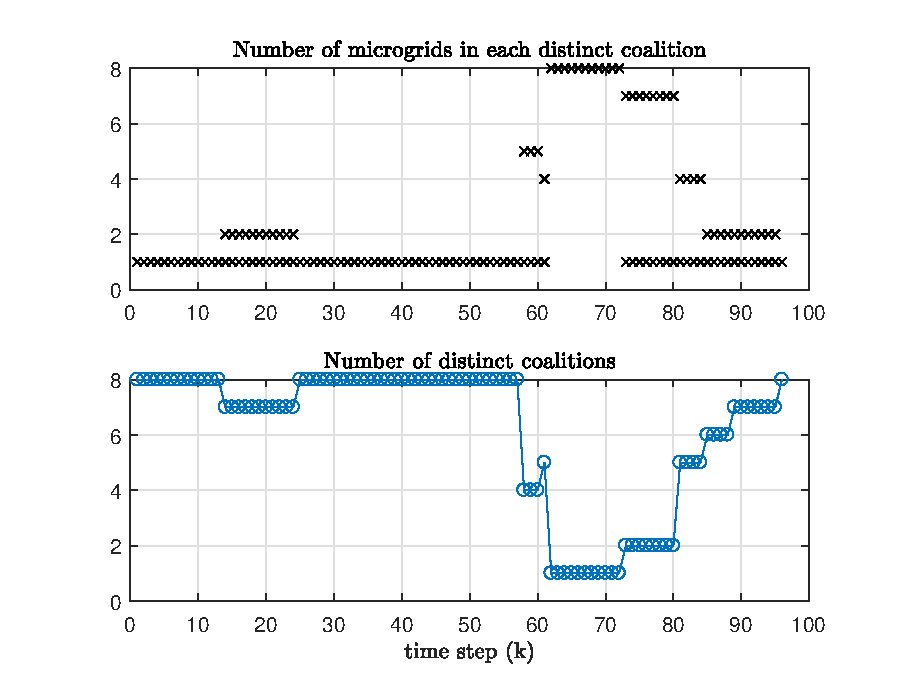
\includegraphics[scale=0.6]{img/co_res.eps}
	\caption{The evolution of coalitions formed.
	}
	\label{fig:co_res}
\end{figure}
\iffalse 
\begin{figure}
	\centering
	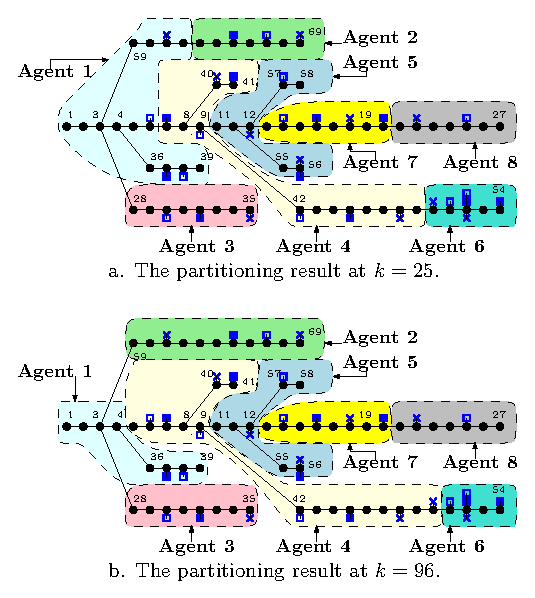
\includegraphics[scale=0.9]{img/part_res.eps}
	\caption{Partitioning results at a. $k=25$ and b. $k=96$. At both time instants, the resulting microgrids are self-sufficient.
	}
	\label{fig:part_res}
\end{figure}
\fi 
\begin{figure}
	\centering
	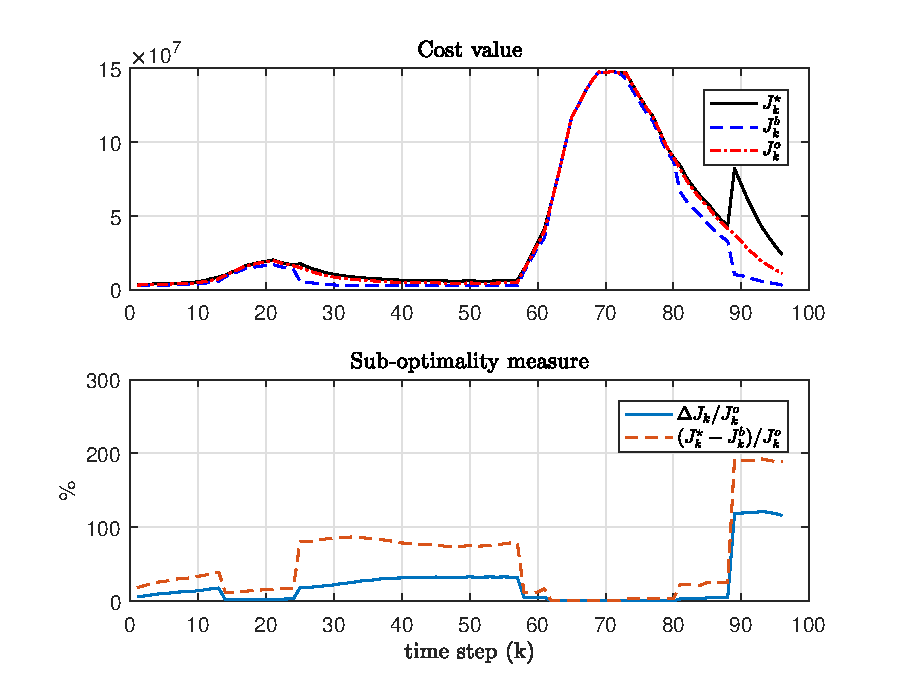
\includegraphics[scale=0.6]{img/delta_J2.eps}
	\caption{Top plot shows the cost values computed using the proposed scheme, $J^{\star}_k$, (solid line), by solving Problem \eqref{eq:MPC_net} centrally as the benchmark $J^{o}_k$, (dashed-dotted line), and the lower bound, $J^{b}_k$ (dashed line). Bottom plot shows the suboptimality of the proposed scheme and its upper bound.
	}
	\label{fig:deltaJ}
\end{figure}

\section{Conclusion and future work}
\label{sec:concl}
We develop a non-centralized MPC-based economic dispatch scheme for systems of interconnected microgrids. The approach consists of an event-triggered repartitioning method with the aim of maintaining self-sufficiency of each microgrid and decomposing the centralized economic dispatch problem into coalition-based sub-problems in order to compute a feasible but possibly sub-optimal decisions. The main advantage of the approach is a low communication burden, which is essential for online applications. %Additionally, the effectiveness of the approach is also showcased in a numerical study. 
%As future work, we would like to combine self-sufficiency and sub-optimality as the criteria that trigger the repartitioning process since we notice in the case study that the sub-optimality measure might change rapidly due to the repartitioning of the network. Therefore, it might be better for the network to maintain the current partition when the performance is highly compromised. In this regard, the repartitioning and coalition formation procedures might also need to be adjusted.
\vspace{-10pt}
\begin{ack}                               % Place acknowledgements
This work has received funding from the European Union's Horizon 2020 research and innovation programme under the Marie Sk\l{}odowska-Curie grant agreement No 675318 (INCITE).  % here.
\end{ack}
\vspace{-10pt}
{%\small 

\bibliographystyle{dcu}        % Include this if you use bibtex 
\bibliography{ref_ja}           % and a bib file to produce the 
}                                % bibliography (preferred). The
                                 % correct style is generated by
                                 % Elsevier at the time of printing.


%\appendix
%\section{A summary of Latin grammar}    % Each appendix must have a short title.
%\section{Some Latin vocabulary}         % Sections and subsections are supported  
                                        % in the appendices.
\end{document}
